%% EAAI first draft converted to Elsevier elsarticle format.
%% Target journal: Engineering Applications of Artificial Intelligence.
\documentclass[preprint,review,12pt,nonatbib]{elsarticle}

\usepackage[utf8]{inputenc}
\usepackage[T1]{fontenc}
\usepackage{amsmath,amssymb,amsfonts}
\usepackage{graphicx}
\usepackage{booktabs}
\usepackage{tabularx}
\usepackage{array}
\usepackage{algorithm}
\usepackage{algpseudocode}
\usepackage{lineno}
\usepackage{xcolor}
\usepackage{newunicodechar}
\newunicodechar{▹}{$\triangleright$}
\newunicodechar{ï}{\"i}
\newunicodechar{Γ}{\Gamma}
\newunicodechar{’}{'}
\newunicodechar{“}{``}
\newunicodechar{”}{''}
\newunicodechar{–}{--}
\newunicodechar{—}{---}
\newunicodechar{−}{-}
\newunicodechar{×}{\times}
\graphicspath{{figures/}}

\usepackage[backend=biber,style=numeric,sorting=none]{biblatex}
\addbibresource{references.bib}

\journal{Engineering Applications of Artificial Intelligence}

\begin{document}
\begin{frontmatter}

\title{Graph-Aware Deep Reinforcement Learning for Adaptive Capacity Planning in Distributed Personalized Regenerative Medicine Manufacturing Networks}

\author[inst1]{Zhaowei Li\corref{cor1}}
\ead{zli686@gatech.edu}
\cortext[cor1]{Corresponding author.}
\author[inst1]{Chin-Yuan Tseng}
% \ead{...}  % add publication email if you want it listed for the second author
\affiliation[inst1]{organization={H. Milton Stewart School of Industrial and Systems Engineering, Georgia Institute of Technology},
            city={Atlanta},
            state={GA},
            country={USA}}

\begin{abstract}

Autologous cell therapy and other personalized regenerative medicine (PRM)
products are manufactured on demand across distributed clinics. Each product
is perishable, identity-bound and non-fungible, and useful only while its
patient remains clinically eligible, coupling capacity, inventory,
patient-indexed logistics, and patient outcomes. We formulate this planning
problem as a constrained graph Markov decision process and develop an
\emph{advantage-filtered residual graph convolutional network--deep deterministic
policy gradient} controller (AFR-GCN--DDPG). It learns bounded corrections to a
transparent two-period look-ahead policy while preserving identity and
feasibility. In the routing-primary formal study, five training seeds were
evaluated on four scenarios with 100 paired holdout replications per seed and
scenario. AFR-GCN--DDPG reduced the total weighted objective by 0.658\% relative
to routing MDL-2 (95\% interval $[-0.721,-0.585]\%$) and by 0.321\% relative to
parameter-matched flat DDPG (95\% interval $[-0.413,-0.240]\%$), while improving
completion service, manufacturing eligibility, and patient loss. Savings were
driven primarily by lower patient-loss, expiry, and shortage costs, partly
offset by higher specimen-transfer cost. A matched three-seed TD3 development
ablation also favored the graph controller over MDL-2 and flat TD3. However,
DDPG and TD3 final checkpoints were statistically indistinguishable from frozen
pretraining, and a prospective paired-advantage DDPG experiment failed its
online-gain gate. Frozen action-geometry screens found that useful local
headroom concentrated in projected integer-lot specimen routing rather than
continuous reagent and capacity channels. The evidence supports an
offline-pretrained, graph-aware residual actor--critic policy, but not an
independent endpoint benefit from the tested online updates.
\end{abstract}

\begin{keyword}
Graph convolutional networks \sep Deep reinforcement learning \sep Actor--critic methods \sep Capacity planning \sep Distributed manufacturing \sep Personalized regenerative medicine \sep Perishable inventory \sep Transshipment
\end{keyword}

\end{frontmatter}
\linenumbers


\section{Introduction}
\label{sec:introduction}

Distributed make-to-order manufacturing networks are increasingly important in engineering systems where products are individualized, production capacity is scarce, and service outcomes depend on time-sensitive sequential decisions. Personalized regenerative medicine (PRM), and autologous cell therapy in particular, is a demanding instance of this class. Each therapy is manufactured from an individual patient's own biological material, so production can begin only when that patient's specimen, an available bioreactor, and sufficient consumables are simultaneously present, and the finished product must be returned to the same patient within a limited viability window. Because the product is patient-specific, it cannot be pre-produced, pooled, or substituted, and the opportunity to buffer against uncertainty with inventory is fundamentally limited~\cite{Wang2023SimulationBased, Zheng2022HybridMBRL}. Three properties therefore distinguish PRM capacity planning from conventional make-to-order or inventory control. The product is \emph{perishable}, subject to a hard shelf-life and vein-to-vein deadline; it is \emph{identity-bound}, tied one-to-one to a single patient and non-fungible across patients; and its demand is driven by \emph{patient health}, since a patient whose condition deteriorates while waiting may become clinically ineligible before treatment can be delivered. These are not marginal concerns. Autologous CAR-T manufacturing has a turnaround measured in weeks, an estimated 4--7\% of patients never receive their product because of manufacturing failure, and in multiple myeloma roughly one quarter of patients die while waitlisted for a BCMA-directed CAR-T production slot~\cite{AyalaCeja2024CARTManufacturing}. Discrete-event simulation links longer waits directly to survival, with predicted one-year mortality in large B-cell lymphoma rising from about 36\% to 76\% as vein-to-vein time increases from one to nine months~\cite{Tully2019WaitTimes}. With the CAR-T market projected to reach tens of billions of US dollars by the early 2030s~\cite{GrandView2024CART}, delivering perishable, patient-specific product before patients deteriorate is a consequential operational challenge.

These properties make capacity planning a coupled, network-level decision problem rather than a collection of independent local ones. Locating production near patients through distributed or point-of-care manufacturing shortens fulfillment time, but it also creates spatial dependencies. A shortage at one clinic can sometimes be relieved by relocating idle bioreactor capacity or transshipping consumables from connected facilities, and each such action changes the future state of the whole network~\cite{Li2023, Tseng2023DeepRL}. Identity binding constrains ownership and use, not physical location: reagents and idle bioreactor capacity are fungible, whereas each specimen lot and finished product remain attached to one named patient. An intact waiting specimen may therefore be routed to a qualified manufacturing facility without being pooled, split, substituted, or reassigned, and the resulting product must return to that patient's collection or infusion site. Coordination must account for this patient-indexed logistics pathway as well as fungible-resource sharing. The state of such a system is naturally relational, since each facility is a node whose value depends on its neighbors' queues and inventories and on the links along which shortages, slack, specimens, and disruptions propagate. A flat feature vector encodes local conditions but discards this topology, which motivates a graph-structured state representation as a matter of substance rather than convenience.

Reinforcement learning (RL) is a natural fit because the problem is sequential. An action taken in one period alters future inventories, capacity, waiting specimens, and service outcomes. Continuous-control actor--critic methods, including deep deterministic policy gradient (DDPG)~\cite{Lillicrap2016DDPG}, twin delayed DDPG (TD3)~\cite{Fujimoto2018TD3}, soft actor--critic (SAC)~\cite{Haarnoja2018SAC}, and proximal policy optimization (PPO)~\cite{Schulman2017PPO}, are standard tools for such real-valued control. Graph convolutional networks (GCNs)~\cite{Kipf2017GCN} provide a permutation-equivariant relational inductive bias for encoding networked state. This machinery is by now well established, and a substantial literature already couples graph learning with reinforcement learning for supply-chain and resource-allocation problems~\cite{Kotecha2025GNNMARL, Chang2025AAAI, Ahn2024GSP, Ahn2024GPP, Liu2024GNNMARLSurvey}. We therefore do not claim novelty in combining graph representation with reinforcement learning.

What that literature does not model is the PRM problem itself. Prior graph-and-RL studies for networked operations concentrate on demand forecasting, inventory-only ordering, or generic enterprise resource allocation, and they represent demand as fungible, abstract requests~\cite{Kotecha2025GNNMARL, Ahn2024GSP, Mousa2023DecInvMARL, Bermudez2023DCPO, Eisenach2024NeuralCoordination}; none model a product that expires, production that must return to the same patient, or demand generated by patient deterioration while waiting. Reinforcement learning has been applied within cell-therapy manufacturing, but at the level of a single bioprocess rather than a network of clinics~\cite{Zheng2022HybridMBRL}, and recent evidence cautions that learned policies do not uniformly dominate well-tuned operational heuristics, particularly under perishability and non-stationarity~\cite{Stranieri2025PharmaDRL}. The gap we address is thus a problem gap rather than a method gap, namely perishable, identity-bound, patient-condition-driven capacity planning across a clinic network, together with a decision framework and simulation testbed built specifically for it. To the best of our knowledge no public benchmark exists for this setting, so the environment is itself a contribution.

We organize the study around five research questions. \textbf{(RQ1)} With patient-indexed specimen routing held admissible across policies, does a graph representation of the clinic network improve coordinated specimen, capacity, reagent, and replenishment decisions over flat-state control, and under which supply-disruption and forecast-error conditions is any improvement largest? \textbf{(RQ2)} Does the routing-primary graph advantage persist under a matched TD3 backbone ablation, and can any gain be attributed separately to online actor--critic updates rather than frozen advantage-filtered pretraining? \textbf{(RQ3)} Does explicitly modeling patient condition and product expiry change the optimal policy and expose failures of condition-blind planners? \textbf{(RQ4)} Does a condition- and expiry-aware temporal encoder, which retains memory of deterioration trajectories, improve on a static graph encoder? \textbf{(RQ5)} Do learned policies outperform strong look-ahead heuristics, not only weak myopic rules, under supply disruption, demand forecast error, and patient-condition stress?

To study these questions we develop, first, a simulation of a multi-site autologous cell-therapy network in which patient health conditions, patient-indexed specimen routing, and product and material expiry are first-class drivers of demand and feasibility, and second, an advantage-filtered residual GCN--DDPG (AFR-GCN--DDPG) controller that coordinates specimen routing, capacity, reagent, and replenishment decisions across the network. AFR is our shorthand for the complete controller design: a transparent MDL-2 anchor, a graph-aware bounded residual actor, evidence-filtered teacher targets, and independently calibrated deployment safeguards. It does not replace or rename DDPG. The graph component encodes each facility's operational and patient-condition state together with information from connected facilities into network-aware embeddings. A deterministic policy-gradient actor then learns a bounded, state-dependent correction to the anchor policy, and a feasibility projection converts the corrected action into implementable controls. Advantage-filtered distillation retains a nonzero correction target only when common-random-number look-ahead predicts an improvement over the anchor; it is a teacher-data construction and regularization step, not a second algorithm or deployed policy. Checkpoint and residual-scale calibration provide a deployment safeguard. DDPG is the canonical proposed instantiation and provides continuity with prior PRM capacity-planning work; a parameter-matched graph-aware TD3 study serves as a development-only backbone ablation, while SAC and PPO remain future common-budget routing-primary comparisons. We adopt a statistically disciplined evaluation protocol (multiple random seeds, paired Monte Carlo outcomes, and two-level confidence intervals), because single-seed, mean-only reporting can make deep reinforcement learning results appear stronger and more stable than they are~\cite{Henderson2018DRLMatters, Agarwal2021RLiable}. Consistent with the clinical stakes of the problem, we report patient-service outcomes such as eligibility and waiting alongside operating cost, since a lower average cost can mask clinically unacceptable delay.

The main contributions of this study are as follows.
\begin{itemize}
    \item We formulate distributed capacity planning for \emph{perishable, identity-bound, patient-condition-driven} PRM manufacturing as a constrained networked sequential decision problem, in which patient deterioration and product and material expiry are explicit determinants of demand, feasibility, and cost.
    \item We develop a simulation environment realizing this formulation for a multi-clinic autologous cell-therapy network, with patient-condition dynamics, expiry-aware inventory, patient-indexed and identity-preserving pre-manufacturing specimen routing, finished-product return, and fungible-resource sharing. Routing is an operational capability of the model rather than a claimed methodological contribution.
    \item We propose AFR-GCN--DDPG, a two-stage advantage-filtered residual graph controller that learns bounded corrections to a transparent look-ahead anchor, retains the filtered teacher signal during DDPG optimization, and applies independently calibrated deployment safeguards.
    \item We establish a paired multi-seed evaluation protocol that separates policy-versus-anchor value, graph-versus-flat representation value, DDPG-versus-TD3 backbone robustness, and final-versus-frozen online attribution. The evidence includes a five-seed formal DDPG confirmation and a matched three-seed TD3 development ablation with two-level bootstrap confidence intervals.
    \item We report prospective negative attribution tests rather than folding all learned-policy performance into an online-RL claim. Paired critic supervision, legal-action transfer diagnostics, and corrected action-geometry screens identify offline advantage-filtered pretraining and graph representation as the supported sources of value, while bounding the unsupported incremental online-update claim.
    \item We draw design implications for intelligent decision support in distributed, patient-specific healthcare manufacturing and related time-critical, make-to-order engineering systems.
\end{itemize}

The remainder of this paper is organized as follows. Section~\ref{sec:problem} formulates the distributed PRM capacity planning problem, extended with patient-condition states and product and material expiry. Section~\ref{sec:literature} reviews personalized regenerative medicine operations, reinforcement- and graph-learning for networked operational decisions, and the method foundations of continuous-control reinforcement learning and graph neural networks, closing with the design implications that motivate our approach. Section~\ref{sec:method} presents the graph-aware deep reinforcement learning framework. Section~\ref{sec:experiments} describes the computational experiments and results. Section~\ref{sec:conclusion} concludes the study and identifies future research directions.

\section{Distributed Network Manufacturing and Capacity Planning Problem}
\label{sec:problem}
\begin{table}[htbp]
\centering
\caption{Notation used in the distributed manufacturing and capacity planning model.}
\label{tab:notation}
\footnotesize
\setlength{\tabcolsep}{4pt}
\renewcommand{\arraystretch}{1.08}
\begin{tabularx}{\textwidth}{>{\raggedright\arraybackslash}p{0.16\textwidth} >{\raggedright\arraybackslash}X}
\toprule
\multicolumn{2}{c}{\textbf{Sets and parameters}} \\
\midrule
$\Gamma$ & Planning horizon indexed by $t$. \\
$T$ & Manufacturing time for one PRM product, in periods, where $T<\Gamma$. \\
$N$ & Set of manufacturing facilities indexed by $n$. \\
$\mathcal{E}_{S}$ & Qualified facility pairs along which an intact waiting specimen lot may be routed before manufacturing. \\
$m_t^n$ & Products that begin manufacturing at facility $n$ at epoch $t$. \\
$d_t^n$ & Demand arrivals at facility $n$ in epoch $t$. \\
\midrule
\multicolumn{2}{c}{\textbf{State variables}} \\
\midrule
$s_t^n$ & Patient-indexed specimens waiting for manufacturing at their current facility $n$ at epoch $t$. \\
$r_t^n$ & Available reagent units at facility $n$ at epoch $t$. \\
$\mathbf{b}_t^n$ & Bioreactor work-in-process vector $(b_t^{n,1}, b_t^{n,2}, \ldots, b_t^{n,T})$, where $b_t^{n,\tau}$ denotes the number of bioreactors at facility $n$ with $\tau$ periods remaining at epoch $t$. \\
$P_t^n$ & Maximum reagent purchase quantity for facility $n$ for epoch $t+1$. \\
\midrule
\multicolumn{2}{c}{\textbf{Decision variables}} \\
\midrule
$w_t^n$ & Executed integer net flow of intact waiting specimen lots into (positive) or out of (negative) facility $n$ at epoch $t$, with identity and network conservation enforced (Section~\ref{sec:problem-identity}). \\
$e_t^n$ & Reagent units added to or subtracted from facility $n$ at epoch $t$ and received or removed before epoch $t+1$. \\
$q_t^n$ & Idle bioreactors added to or subtracted from facility $n$ at epoch $t$ and received or removed before epoch $t+1$. \\
$p_t^n$ & Reagent purchase quantity for facility $n$ for epoch $t+1$. \\
\midrule
\multicolumn{2}{c}{\textbf{Patient-condition and perishability}} \\
\midrule
$H_j$ & Latent health index of patient $j$, drawn $H_j \sim \mathrm{Uniform}(0,1)$ at enrollment. \\
$\tau_j$ & Deterioration epoch of patient $j$, drawn $\tau_j \sim \theta\,\mathrm{Weibull}(\kappa)$. \\
$\kappa,\theta$ & Shape and scale of the Weibull deterioration-epoch distribution. \\
$\alpha_j$ & Number of epochs since patient $j$ enrolled, including waiting and manufacturing time. \\
$S_j$ & Survival index of patient $j$, $S_j \in [0,1]$; the patient is eligible while $S_j \ge \epsilon$. \\
$\lambda_H,\lambda_F$ & Survival decay rates of an ideally healthy and a maximally frail patient, with $\lambda_H < \lambda_F$. \\
$\rho$ & Post-deterioration acceleration factor for effective exposure time, $\rho > 1$. \\
$\epsilon$ & Eligibility threshold on the survival index. \\
$\delta$ & Urgency margin defining at-risk patients ($S_j < \epsilon + \delta$). \\
$\ell_{\mathrm{mat}},\ell_{\mathrm{fin}}$ & Shelf lives, in epochs, of source material and finished product. \\
$\boldsymbol{\sigma}_t^n$ & Condition and routing summary at facility $n$: waiting-queue survival bands, in-transit arrivals, route eligibility, and in-production condition risk. \\
$\phi_t^n$ & Patients lost at facility $n$ in epoch $t$ through waiting, transit, manufacturing, return, or expiry events. \\
$\psi_t^n$ & Specimens, in-process therapies, and finished units wasted at facility $n$ in epoch $t$. \\
$\upsilon_t^n$ & At-risk unserved patients at facility $n$ in epoch $t$. \\
$\omega_{\mathrm{lost}},\omega_{\mathrm{exp}},\omega_{\mathrm{urg}}$ & Cost weights for patient loss, material waste, and urgency, with $\omega_{\mathrm{lost}} \gg \omega_{\mathrm{exp}} > \omega_{\mathrm{urg}}$. \\
\bottomrule
\end{tabularx}
\end{table}


In this section, we formulate the capacity planning problem for distributed manufacturing systems as a production simulation model based on a Markov decision process (MDP). Suppose the distributed manufacturing system consists of $N$ manufacturing facilities that produce one type of make-to-order PRM product. Each manufacturing facility has its own production capacity, including bioreactors and reagent inventory, and can purchase reagents from source material suppliers. Facilities receive patient-indexed specimens and initiate production when the matched specimen, an available bioreactor, and sufficient reagents are co-located. Reagent transshipment and idle-bioreactor relocation are allowed among qualified facilities. In addition, one intact waiting specimen lot may be routed before manufacturing without changing the patient--specimen association; pooling, splitting, substitution, cross-patient use, and in-process transfer remain prohibited, and finished product is returned to the same patient's collection site (Section~\ref{sec:problem-identity}). Demand arrivals and supplier disruptions are modeled as stochastic processes, implying that local supply may be either insufficient or excessive relative to local demand at different decision epochs. The notation used throughout this section is summarized in Table~\ref{tab:notation}.

Figure~\ref{fig:manufacturing_system} illustrates the basic structure of the distributed manufacturing problem using a two-facility example. Each facility maintains a patient--specimen queue whose members carry a deteriorating survival index, together with reagent inventory, bioreactor capacity, and perishable finished product. At each decision epoch, condition-driven patient demand and disruption-prone reagent replenishment arrive under uncertainty. When one facility experiences excess demand, insufficient reagents, or limited production capacity, the network may transship reagents, relocate idle bioreactors, or route an intact waiting specimen to a qualified manufacturing facility. The latter is patient-indexed logistics rather than sharing: identity, ownership, and the final infusion destination never change. This structure motivates the MDP formulation, where the state captures facility-level demand, patient condition, material location and transit, inventory, and capacity, and the action coordinates both patient-indexed routing and fungible-resource decisions.

\begin{figure}[htbp]
    \centering
    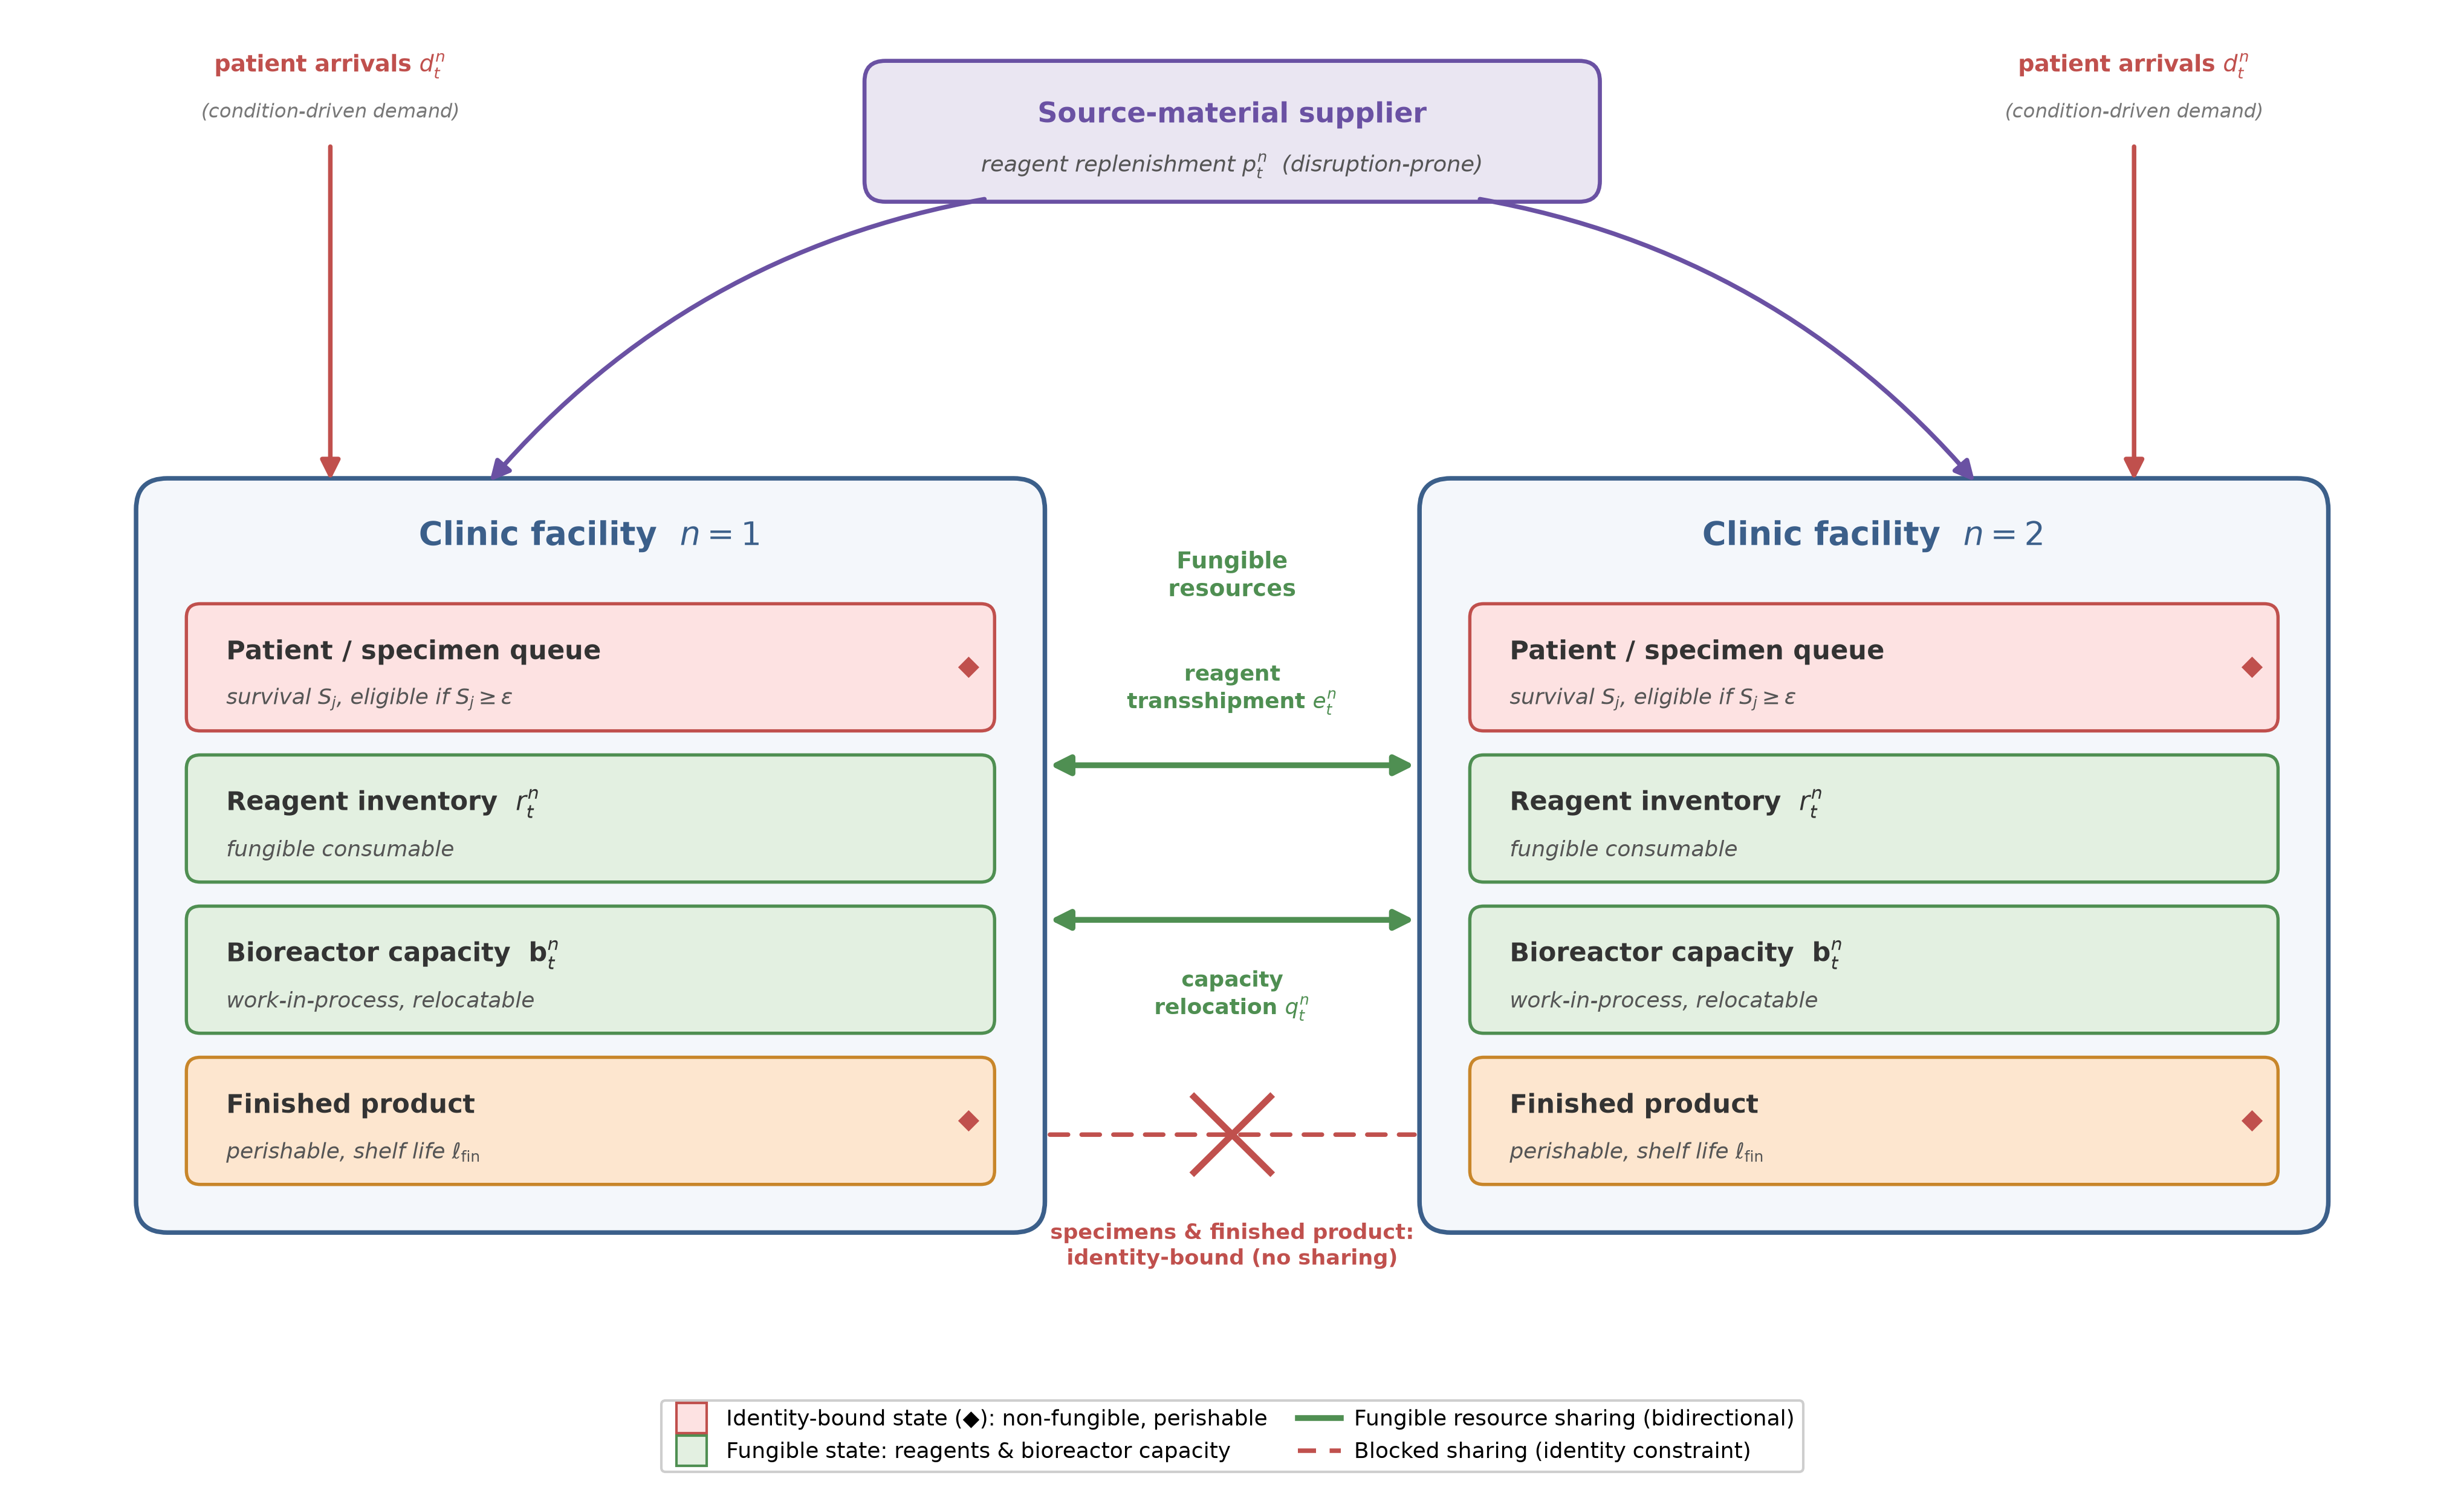
\includegraphics[width=0.95\textwidth]{figures/Figure 1.png}
    \caption{Illustration of a two-facility distributed manufacturing system for personalized regenerative medicine. Each facility holds a patient--specimen queue whose members carry a deteriorating survival index $S_j$ (eligible while $S_j \ge \epsilon$), reagent inventory $r_t^n$, bioreactor capacity $\mathbf{b}_t^n$, and perishable finished product. Condition-driven patient demand $d_t^n$ and disruption-prone reagent replenishment $p_t^n$ arrive under uncertainty. Reagents and idle bioreactor capacity are fungible and can be rebalanced through transshipment $e_t^n$ and relocation $q_t^n$ (solid green links). The crossed red link denotes prohibited pooling, substitution, or cross-patient reassignment of specimens and products; it does not prohibit identity-preserving transport of one intact waiting specimen lot to a qualified manufacturing facility or return of its product to the same patient.}
    \label{fig:manufacturing_system}
\end{figure}

For the $N$ facilities, $T$ epochs of manufacturing time are required to produce one of the PRM products, and the planning horizon consists of $\Gamma$ epochs where $\Gamma>T$.

At epoch $t \in\{1,2, \cdots, \Gamma\}$, the production status of the $n$-th facility for $n=1, \cdots, N$ is expressed as a state vector $\mathbf{x}_{t}^{n}$, where

\begin{equation}
\mathbf{x}_{t}^{n}=\left(s_{t}^{n}, r_{t}^{n}, \mathbf{b}_{t}^{n}, P_{t}^{n}\right),
\end{equation}
Based on the state variables at epoch $t$, the facilities need to take action to adjust their production capacity for epoch $t+1$. We define the action $\mathbf{a}_{t}^{n}$ as a vector that consists of the amount of capacity sharing and reagent replenishment. The action is decided at the beginning of the production period $t$ and executed before the start of $t+1$.

\begin{equation}
\mathbf{a}_{t}^{n}=\left(w_{t}^{n}, e_{t}^{n}, q_{t}^{n}, p_{t}^{n}\right),
\end{equation}

The goal of capacity planning is to minimize total production cost by dynamically selecting the actions from Equation (2) for all facilities, denoted by $\mathbf{A}_{t}=\left(\mathbf{a}_{t}^{1}, \cdots, \mathbf{a}_{t}^{N}\right)$, for each epoch $t \in \Gamma$. We define $V\left( \mathbf{X}_{t}\right)$ as the total future cost of the selecting actions $\mathbf{A}_{t}$ when the states from all facilities, denoted by $\mathbf{X}_{t}=\left(\mathbf{x}_{t}^{1}, \cdots, \mathbf{x}_{t}^{N}\right)$, are observed at epoch $t \in \Gamma$. The objective function can be expressed as a dynamic programming problem:

\begin{equation}
\begin{array}{ll}
 V\left( \mathbf{X}_{t}\right)= 
 \min _{\mathbf{A}_{t}} & E\left[c\left(\mathbf{A}_{t} ; \mathbf{X}_{t}\right)+\gamma  V\left(\mathbf{X}_{t+1}\right)\right],
\end{array}
\end{equation}

which is useful for finding the optimal action $\mathbf{A}_{t}$ for each state $\mathbf{X}_{t}$ at each epoch $t \in \Gamma$, where $c\left(\mathbf{A}_{t} ; \mathbf{X}_{t}\right)$ is the immediate cost at time $t$, and $\gamma \in[0,1]$ is a discount factor for balancing the impact of future costs in deciding actions. The choice of $\gamma$ depends on the user's goal; if $\gamma$ is closer to 1 (to 0 ), then it means the user cares more about long (short) term cost; if $\gamma=0$, then only the cost for current epoch is considered. Equation (3) generalizes the optimality equation for the capacity planning problem in $\mathrm{Li}(2021)$ \cite{Li2023} in that cost functions \textit{$\mathbf{c}$} and $\mathbf{V}$ and the cumulative distribution function for the expectation operator can be unknown.

Equations~(1)--(3) describe the base operational MDP shared with generic networked replenishment problems. The remainder of this section extends it along the three dimensions that distinguish PRM capacity planning, namely the deteriorating clinical condition of the patients awaiting treatment, the hard expiry of biological source material and finished product, and the autologous identity constraint that forbids pooling of patient-specific specimens. Section~\ref{sec:method} then develops a graph-aware DRL approach that learns the cost function $\mathbf{c}$, the value function $\mathbf{V}$, and the expectation operator directly from simulated experience.

\subsection{Patient condition and treatment eligibility}
\label{sec:problem-patient}

In generic capacity planning, a unit of unmet demand is deferred, backordered, or lost at a fixed penalty, and its value does not change while it waits. PRM demand behaves differently, because each arrival is a patient whose clinical condition deteriorates throughout the vein-to-vein pathway. A specimen that waits or travels too long, or a therapy whose matched patient deteriorates during manufacturing or product return, may no longer produce a deliverable treatment. We therefore attach an explicit condition process to every enrolled patient from queue entry through specimen transit, manufacturing, and product return, adapting the real-time patient-health modeling of Tseng et al.~\cite{Tseng2024PatientHealth} to a distributed capacity-planning setting.

When a patient $j$ enrolls at facility $n$, we draw a latent health index $H_j \sim \mathrm{Uniform}(0,1)$ and a deterioration epoch $\tau_j \sim \theta\,\mathrm{Weibull}(\kappa)$ with shape $\kappa$ and scale $\theta$; $H_j$ captures the heterogeneous baseline robustness across patients, while $\tau_j$ marks the onset of accelerated decline. Let $\alpha_j$ be the number of epochs since enrollment, including both queueing and manufacturing time. The patient's survival index $S_j \in [0,1]$ (a normalized proxy for the likelihood that the patient remains treatable) evolves as

\begin{equation}
\label{eq:survival}
S_j(\alpha_j) = \ell(\alpha_j) + H_j\big(u(\alpha_j) - \ell(\alpha_j)\big),
\end{equation}
where $u(\alpha)=\exp\!\big(-\lambda_H\,g(\alpha)\big)$ and $\ell(\alpha)=\exp\!\big(-\lambda_F\,g(\alpha)\big)$ are the survival trajectories of an ideally healthy and a maximally frail patient, with decay rates $\lambda_H < \lambda_F$, so that $H_j$ interpolates each patient between the two bounds. The effective exposure time

\begin{equation}
\label{eq:effective-time}
g(\alpha) =
\begin{cases}
\alpha, & \alpha \le \tau_j,\\[2pt]
\tau_j + \rho\,(\alpha - \tau_j), & \alpha > \tau_j,
\end{cases}
\end{equation}
accelerates by a factor $\rho > 1$ once the patient passes the deterioration epoch $\tau_j$, reflecting the clinically observed transition to rapid decline. A patient remains eligible for treatment only while $S_j \ge \epsilon$. Before production starts, crossing the threshold removes the patient and specimen from either the waiting or transit state. After production starts, the same condition process continues through manufacturing and any modeled product-return epochs. If the matched patient becomes ineligible before completion, the in-process therapy is discarded and the occupied bioreactor is cleaned during that epoch before returning to the idle pool at the next decision epoch. Treatment service is recorded only when the finished product reaches and is assigned to the original patient, not when production starts. Because condition erodes monotonically in expectation and accelerates after $\tau_j$, waiting, specimen transit, manufacturing, and product-return delay are not neutral buffering decisions. Parameter values are reported in Section~\ref{sec:experiments}.

\subsection{Perishability of materials and finished product}
\label{sec:problem-expiry}

Both the biological source material and the finished product are perishable and identity-specific, so they cannot be stockpiled against future demand. A waiting or in-transit specimen that is not put into production within $\ell_{\mathrm{mat}}$ epochs of enrollment expires, so the patient is lost and the reserved material is wasted. Finished product that is not delivered within $\ell_{\mathrm{fin}}$ epochs of completion likewise expires and is discarded. We track, per facility $n$ and epoch $t$, patients lost to waiting-stage ineligibility $\phi^{n,\mathrm{wait}}_t$, manufacturing-stage ineligibility $\phi^{n,\mathrm{mfg}}_t$, return-stage ineligibility $\phi^{n,\mathrm{ret}}_t$, local specimen expiry $\phi^{n,\mathrm{exp}}_t$, transit ineligibility $\phi^{n,\mathrm{tr\text{-}inel}}_t$, transit expiry $\phi^{n,\mathrm{tr\text{-}exp}}_t$, and modeled transit loss $\phi^{n,\mathrm{tr\text{-}loss}}_t$, together with finished units lost to expiry $\psi^{n,\mathrm{fin}}_t$. A manufacturing-stage ineligibility also creates one discarded in-process therapy. It is convenient to collect the total patients lost and total material wasted at each facility,

\begin{equation}
\label{eq:loss-aggregates}
\begin{aligned}
\phi^{n}_t ={}& \phi^{n,\mathrm{wait}}_t + \phi^{n,\mathrm{mfg}}_t
  + \phi^{n,\mathrm{ret}}_t + \phi^{n,\mathrm{exp}}_t \\
&+ \phi^{n,\mathrm{tr\text{-}inel}}_t + \phi^{n,\mathrm{tr\text{-}exp}}_t
  + \phi^{n,\mathrm{tr\text{-}loss}}_t, \\
\psi^{n}_t ={}& \phi^{n,\mathrm{exp}}_t + \phi^{n,\mathrm{mfg}}_t
  + \phi^{n,\mathrm{tr\text{-}exp}}_t \\
&+ \phi^{n,\mathrm{tr\text{-}loss}}_t + \psi^{n,\mathrm{fin}}_t,
\end{aligned}
\end{equation}
where an expired or lost specimen contributes both a lost patient and a unit of wasted material. To signal impending losses before they occur, we also count the \emph{at-risk unserved} patients whose survival has fallen within an urgency margin $\delta$ of the eligibility boundary, $\upsilon^{n}_t = \big|\{\, j \text{ waiting at } n : S_j < \epsilon + \delta \,\}\big|$.

\subsection{Autologous identity constraint and admissible transfers}
\label{sec:problem-identity}

The autologous nature of PRM imposes a constraint with no analog in commodity supply chains. A specimen and the product manufactured from it are bound to one patient and cannot be substituted, pooled, split, or delivered to anyone else. Identity preservation does not, however, require the source material to remain at its collection site. We therefore allow \emph{patient-indexed, identity-preserving, pre-manufacturing specimen routing}: only a complete lot in the waiting state may move, only along a qualified edge in $\mathcal{E}_{S}$, and at most once by a direct route before manufacturing begins. Multi-hop routing, cycles, in-production transfer, cross-patient consumption, and product reassignment are prohibited.

The aggregate decision $w_t^n$ records the executed integer net flow produced by a patient-level routing executor. The executor pairs facilities with opposite signed requests, selects eligible waiting identities deterministically, and conserves lots so that $\sum_n w_t^n=0$. Each selected patient's immutable identity record retains the collection facility, current material location, manufacturing facility, and transfer history. The main routing setting dispatches at epoch $t$, advances condition and specimen age once during one transit epoch, and makes the lot available before the epoch $t+1$ production decision. After off-site manufacturing, the finished product remains assigned to the same patient and is returned to that patient's collection or infusion facility. Thus, routing changes manufacturing location without creating unrestricted specimen sharing.

\subsection{Extended cost and the constrained graph MDP}
\label{sec:problem-graph-mdp}

The immediate cost augments the operational base cost $c_{\mathrm{op}}$ (covering reagent purchase, holding, and shortage; bioreactor holding and shortage; and reagent and capacity transfer) with three condition- and perishability-driven terms:

\begin{equation}
\label{eq:cost}
c(\mathbf{A}_t;\mathbf{X}_t) = c_{\mathrm{op}}(\mathbf{A}_t;\mathbf{X}_t)
+ \omega_{\mathrm{lost}}\!\sum_{n\in N}\phi^n_t
+ \omega_{\mathrm{exp}}\!\sum_{n\in N}\psi^n_t
+ \omega_{\mathrm{urg}}\!\sum_{n\in N}\upsilon^n_t,
\end{equation}
with weights ordered $\omega_{\mathrm{lost}} \gg \omega_{\mathrm{exp}} > \omega_{\mathrm{urg}}$ to encode the clinical priority, in which losing a patient dominates wasting material, which in turn dominates the shaping penalty for letting patients drift toward the eligibility boundary. The urgency term $\upsilon^n_t$ steers the controller to act pre-emptively (starting production or relocating capacity) before losses are actually incurred.

For clarity, we distinguish three quantities throughout the paper. For a policy
$\pi$, the expected total weighted objective is
\begin{equation}
\label{eq:episode-objective}
J^{\pi}_{\mathrm{tot}}
=
\mathbb{E}_{\pi}\!\left[
\sum_{t=0}^{\Gamma-1}c(\mathbf{A}_t;\mathbf{X}_t)
\right]
=
J^{\pi}_{\mathrm{op}}+J^{\pi}_{\mathrm{pat}},
\end{equation}
where $J^{\pi}_{\mathrm{op}}$ accumulates reagent purchase, holding, and
shortage; bioreactor holding and shortage; and reagent and capacity transfer,
whereas $J^{\pi}_{\mathrm{pat}}$ accumulates the weighted patient-loss, expiry,
and urgency terms in Equation~\eqref{eq:cost}. The total objective is the
primary optimization and evaluation criterion. The two component groups are
reported separately to show which decisions generate an improvement.

All three quantities are reported in \emph{modeled weighted-objective units}.
Resource-price coefficients can be interpreted as monetary equivalents under
the adopted calibration, but the patient-loss, expiry, and urgency weights are
penalty or shadow-value parameters rather than observed accounting
expenditures. Consequently, an absolute difference in
$J_{\mathrm{tot}}$ is not presented as realized cash savings without an
external economic calibration. Some large components are driven partly by
exogenous demand and patient deterioration and by structural constraints such
as finite capacity and lead times. They are therefore only partly controllable,
not ``fixed'' or wholly unavoidable.

For an anchor policy $\pi_{\mathrm{anc}}$ and candidate $\pi$, the headline
relative improvement retains the complete objective as its denominator,
\begin{equation}
\label{eq:relative-total-improvement}
R_{\mathrm{tot}}
=
\frac{J^{\pi_{\mathrm{anc}}}_{\mathrm{tot}}
-J^{\pi}_{\mathrm{tot}}}
{J^{\pi_{\mathrm{anc}}}_{\mathrm{tot}}}.
\end{equation}
We accompany it with absolute paired differences, component-specific relative
changes, and clinical outcomes. When a valid oracle or lower-cost reference
$\pi_{\mathrm{ref}}$ is available, we additionally report the fraction of
anchor headroom captured,
\begin{equation}
\label{eq:headroom-captured}
R_{\mathrm{headroom}}
=
\frac{J^{\pi_{\mathrm{anc}}}_{\mathrm{tot}}
-J^{\pi}_{\mathrm{tot}}}
{J^{\pi_{\mathrm{anc}}}_{\mathrm{tot}}
-J^{\pi_{\mathrm{ref}}}_{\mathrm{tot}}}.
\end{equation}
This decomposition prevents a large patient-penalty or capacity-shortage
component from obscuring a meaningful change in a directly affected operating
component, while avoiding a post hoc replacement of the primary denominator.

To act on this cost, the controller needs visibility into the condition of each waiting queue. We therefore extend the facility state of Equation~(1) with a condition summary $\boldsymbol{\sigma}^n_t$,

\begin{equation}
\label{eq:extended-state}
\tilde{\mathbf{x}}^n_t = \big(s^n_t, r^n_t, \mathbf{b}^n_t, P^n_t, \boldsymbol{\sigma}^n_t\big),
\end{equation}
where $\boldsymbol{\sigma}^n_t$ contains the waiting count, waiting mean survival, near-expiry count, waiting survival-band histogram, specimens in transit to the facility, their mean survival, transferred specimens waiting at the facility, route-eligible waiting specimens, in-production count, in-production mean survival, and in-production at-risk count. The controller can therefore anticipate queue, transit, and manufacturing risk rather than merely react to aggregate demand.

Finally, we cast the extended problem as a \emph{constrained graph MDP}. The facilities and their admissible information, reagent, capacity, and specimen-logistics links form a graph $\mathcal{G}=(N,\mathcal{E})$, with the qualified specimen edge set $\mathcal{E}_{S}\subseteq\mathcal{E}$ enforced separately from fungible-resource feasibility. The global state $\tilde{\mathbf{X}}_t=(\tilde{\mathbf{x}}^1_t,\ldots,\tilde{\mathbf{x}}^N_t)$ is a signal over the nodes of $\mathcal{G}$, and the action $\mathbf{A}_t$ assigns per-node purchases, fungible-resource transfers, and conserved patient-indexed specimen-routing requests. The optimality equation~(3) carries over verbatim with the extended state $\tilde{\mathbf{X}}_t$ and cost~\eqref{eq:cost}, but the value function must now trade current operating and logistics cost against the future risk of waiting, transit, patient loss, and expiry. This constrained graph MDP (perishable, identity-bound, and patient-condition-driven) is the problem the remainder of the paper addresses, and its graph structure is precisely what the method of Section~\ref{sec:method} is designed to exploit.


\section{Literature Review}
\label{sec:literature}

We review three bodies of work that our approach draws together, namely the operations of personalized regenerative medicine (PRM) and decentralized manufacturing; reinforcement learning and graph learning for networked operational decisions; and the underlying method foundations of continuous-control reinforcement learning and graph neural networks. Rather than surveying each exhaustively, we read them as an argument in which each stream supplies part of what a distributed PRM capacity-planning controller needs, none supplies all of it, and together they imply a small set of design choices that we make explicit at the end of the section. Throughout, we treat the learning machinery as established and concede that graph representation and reinforcement learning have already been combined for supply-chain problems; what remains open is the PRM problem itself, one that is perishable, identity-bound, and patient-condition-driven.

\subsection{Personalized regenerative medicine and decentralized manufacturing}
PRM supply chains differ substantially from conventional make-to-stock manufacturing systems because products are individualized, time-sensitive, and tightly coupled with patient-specific clinical pathways. In autologous cell therapy, patient material must be collected, transported, manufactured, quality-tested, and returned for administration, and manufacturing can begin only when a specimen, consumables, and production capacity are jointly available. These characteristics make fulfillment time, service reliability, and resource utilization central operational measures. Wang et al.~\cite{Wang2023SimulationBased} used simulation to compare centralized and point-of-care autologous cell therapy supply chain strategies and evaluated cost, fulfillment time, service level, and resource utilization. Li and White~\cite{Li2023} further studied decentralized autologous cell therapy manufacturing networks and showed that transshipment and relocatable capacity can reduce the cost of resilience under supplier disruption. Most directly relevant to our patient-condition modeling, Tseng et al.~\cite{Tseng2024PatientHealth} integrated real-time patient health data into an autologous cell-therapy simulation and showed that representing patient condition, rather than treating demand as static, changes fulfillment and eligibility outcomes. We adopt this patient-condition perspective as a first-class driver of demand and feasibility, but embed it within a networked capacity-planning formulation solved by graph-aware learned control, rather than evaluating fixed policies in a simulation study alone.

These studies establish that PRM network design and inter-facility coordination are first-order engineering decisions rather than implementation details. Related work on cell therapy manufacturing process control also highlights the potential of reinforcement learning in uncertain, nonlinear, and partially observed manufacturing environments~\cite{Zheng2022HybridMBRL}. Together, this literature motivates a data-driven decision-support framework that can represent both the temporal dynamics of patient-specific manufacturing and the spatial dependencies created by distributed facilities.

\subsection{Reinforcement learning for supply chain and manufacturing decisions}
Reinforcement learning has been widely studied for sequential supply chain and manufacturing decisions. Early work applied RL to inventory replenishment in multi-echelon supply chains and perishable inventory systems~\cite{GIANNOCCARO2002153,KARA2018150}. More recent studies have used deep reinforcement learning to handle high-dimensional state spaces, stochastic demand, and simulation-based decision environments. For example, Oroojlooyjadid et al.~\cite{Oroojlooyjadid2022BeerGame} developed a deep Q-network approach for the beer game, demonstrating that DRL can learn replenishment policies in decentralized, partially observed supply chain settings.

Recent supply chain RL studies have moved toward more realistic constraints and engineering settings. Bermudez et al.~\cite{Bermudez2023DCPO} proposed distributional constrained reinforcement learning for multi-period supply chain optimization with production and inventory constraints. Eisenach et al.~\cite{Eisenach2024NeuralCoordination} studied shared-resource capacity control in inventory management using a neural coordination mechanism and a reinforcement learning buying policy. Stranieri et al.~\cite{Stranieri2025PharmaDRL} benchmarked classical and deep reinforcement learning inventory policies for pharmaceutical supply chains with perishability and non-stationary demand. These studies support the use of simulation-trained RL policies for uncertain operational control, but most focus on replenishment or inventory management rather than the joint capacity, reagent, and replenishment decisions (under a perishable, identity-bound demand process) that arise in distributed PRM manufacturing.

\subsection{Structure-informed, residual, and baseline-relative reinforcement learning}
Inventory-control evidence does not support treating generic end-to-end DRL as
automatically superior to established operating rules. Gijsbrechts et
al.~\cite{Gijsbrechts2022InventoryDRL} found that carefully tuned DRL can match
state-of-the-art policies across lost-sales, dual-sourcing, and multi-echelon
problems, while the invited roadmap of Boute et
al.~\cite{Boute2022InventoryRoadmap} argues that learning methods should exploit
the structural policy knowledge accumulated in inventory research. De Moor et
al.~\cite{DeMoor2022RewardShaping} made this principle operational by using
strong perishable-inventory heuristics as teacher policies for reward shaping,
improving training speed, stability, and, in suitable instances, performance
relative to the teacher. Hybrid decomposition offers another route: Stranieri
et al.~\cite{Stranieri2024HybridInventory} assigned production decisions to DRL
and shipping decisions to stochastic programming, obtaining more reliable
performance than pure DRL. Non-stationary-demand experiments further show the
value of conditioning policies on forecast information rather than assuming a
fixed arrival law~\cite{Dehaybe2024NonstationaryInventory}.

Residual reinforcement learning provides the most direct methodological
foundation for our controller. The residual formulation decomposes the
executed action into a competent base-controller action and a learned
correction, reducing the part of the control law that must be discovered from
experience~\cite{Johannink2019ResidualRL}. Staessens et
al.~\cite{Staessens2022ConstrainedResidual} showed in an industrial-control
setting that bounding the correction relative to a conventional controller can
preserve its stabilizing role while adapting to uncertain operating
conditions. Baseline-relative policy-improvement methods likewise motivate
accepting a learned update only when there is credible evidence of improvement
over the incumbent policy~\cite{Metelli2021SafePolicyIteration}. In stochastic
inventory control, Deep Controlled Learning combines approximate policy
iteration with common random numbers and statistically efficient candidate
selection to overcome the difficulty generic DRL has in beating strong
heuristics~\cite{Temizoz2025DeepControlledLearning}. These ideas motivate our
MDL-2 anchor, bounded graph residual, common-random-number advantage filtering,
and held-out deployment calibration. Our validation fallback is an empirical
deployment safeguard, however, and should not be interpreted as inheriting the
formal monotonic-improvement or closed-loop stability guarantees proved under
the assumptions of those methods.

\subsection{Deep reinforcement learning for regenerative medicine capacity planning}
The closest antecedent to this work is Tseng et al.~\cite{Tseng2023DeepRL}, who developed a deep reinforcement learning approach for dynamic capacity planning in decentralized regenerative medicine supply chains. Their study demonstrated that simulation-trained policies can adapt to demand and supply uncertainty without requiring exact prior knowledge of the underlying stochastic processes. This is directly aligned with the objective of using data-driven policy learning for PRM capacity planning.

The present study builds on this line of work by adding an explicit graph representation layer to encode inter-facility relationships. In decentralized PRM networks, facilities are linked through reagent transshipment, idle-bioreactor relocation, and qualified patient-indexed specimen logistics, while every specimen and finished product remains bound to one patient. Therefore, a facility's decision depends not only on its own local state but also on the states, route-eligible queues, transit pipeline, and fungible-resource conditions of connected facilities. A flat vectorized state representation can include all facility variables, but it does not explicitly exploit the graph structure that governs how information, material, and resources propagate across the network. This motivates integrating graph convolutional representation learning with continuous-control actor--critic reinforcement learning.

\subsection{Multi-agent reinforcement learning and graph learning for networked supply chains}
Recent multi-agent reinforcement learning studies are relevant because distributed manufacturing networks naturally involve decentralized information and coordinated actions. Mousa et al.~\cite{Mousa2023DecInvMARL} formulated decentralized inventory control as a multi-agent problem and studied centralized-training/decentralized-execution policies under local information constraints. Leluc et al.~\cite{Leluc2023MARLIM} similarly demonstrated the promise of cooperative multi-agent reinforcement learning for inventory management under stochastic demand and lead times. These studies show that decentralization is not only an application feature but also an algorithmic design dimension.

In parallel, graph neural networks have emerged as a natural representation tool for supply chains and other networked operational systems. Chang et al.~\cite{Chang2025AAAI} learned production functions on supply-chain graphs using temporal graph neural networks and an inventory module, showing the value of explicit relational structure for supply-chain inference and forecasting. Ahn et al.~\cite{Ahn2024GSP} used attention-based graph neural networks for probabilistic supply and inventory prediction in enterprise supply-chain networks, while Ahn et al.~\cite{Ahn2024GPP} combined graph neural networks, offline reinforcement learning, and policy simulation for dynamic supply planning. Kotecha and del Rio Chanona~\cite{Kotecha2025GNNMARL} provide the closest graph-control antecedent: their GNN--MARL framework dynamically parameterizes heuristic inventory policies and uses graph structure to coordinate decentralized supply-chain agents. AFR-GCN--DDPG differs by learning a bounded continuous correction around a fixed look-ahead anchor, filtering correction targets through common-random-number look-ahead, and controlling patient-condition, capacity, fungible-resource, and patient-indexed specimen-routing decisions in an identity-bound PRM network rather than inventory replenishment alone. These studies collectively suggest that graph-based learning is useful for networked supply chain systems; however, most existing work remains focused on prediction, inventory-only control, or general supply-chain planning rather than continuous-action control of PRM-specific capacity, reagent, and specimen flows.

\subsection{Method foundations: continuous-control reinforcement learning and graph neural networks}
The actor proposes real-valued pressures for capacity relocation, reagent replenishment and transfer, and specimen routing; a deterministic executor converts those pressures into feasible mixed continuous and integer decisions. This points to continuous-control actor--critic methods coupled with explicit projection. Deterministic policy gradients and DDPG~\cite{Lillicrap2016DDPG} extended actor--critic learning to continuous action spaces, but are known to suffer from value overestimation and training instability. TD3~\cite{Fujimoto2018TD3} mitigates overestimation through clipped double-$Q$ learning, delayed policy updates, and target smoothing; SAC~\cite{Haarnoja2018SAC} adds entropy regularization for more robust exploration and stability; and PPO~\cite{Schulman2017PPO} is a widely used on-policy alternative built on a clipped surrogate objective. The practical implication is that DDPG, though historically the default for continuous supply-chain control, is no longer an uncontested choice. A defensible study should compare backbones rather than commit to one, and should expect the more stable off-policy methods to reduce the run-to-run variance that plagues DDPG.

Graph neural networks encode relational structure through neighborhood aggregation. The graph convolutional network~\cite{Kipf2017GCN} and its successors (GraphSAGE~\cite{Hamilton2017GraphSAGE} for inductive neighborhood sampling and graph attention networks~\cite{Velickovic2018GAT} for learned edge weighting) provide a permutation-equivariant inductive bias that a flat multilayer perceptron lacks. Coupling such encoders with reinforcement learning has become a recognized paradigm for networked decision problems~\cite{Liu2024GNNMARLSurvey}. For a clinic network whose facilities interact through patient-indexed specimen logistics, capacity relocation, and consumable transshipment, this relational bias is a modeling choice of substance rather than convenience, because it allows a single policy to reason over the topology along which patients, shortages, slack, and disruptions propagate.

\subsection{Evaluation considerations for deep reinforcement learning}
Evaluation rigor is especially important for DRL-based engineering applications. Henderson et al.~\cite{Henderson2018DRLMatters} showed that deep reinforcement learning results can be sensitive to random seeds, hyperparameters, and implementation details. Agarwal et al.~\cite{Agarwal2021RLiable} further argued that few-run comparisons can be statistically unreliable and recommended more robust aggregate metrics and interval estimates. These findings imply that a DRL-based supply chain study should report implementation details, training budgets, out-of-sample test procedures, and variability across replications or random seeds when possible. In the present study, we therefore emphasize common simulation settings across all benchmark policies, detailed implementation parameters for the graph-aware actor--critic agents, and Monte Carlo evaluation under multiple disruption and demand forecast scenarios, with interquartile-mean performance and confidence intervals reported across random seeds.

\begin{table}[htbp]
\centering
\footnotesize
\caption{Positioning of this study relative to closely related literature.}
\label{tab:lit_positioning}
\setlength{\tabcolsep}{3pt}
\renewcommand{\arraystretch}{1.0}
\begin{tabularx}{\textwidth}{p{0.20\textwidth} p{0.25\textwidth} X}
\toprule
Literature stream & Representative studies & Main limitation relative to this work \\
\midrule
PRM operations & Simulation and decentralized planning~\cite{Wang2023SimulationBased,Li2023,Tseng2023DeepRL} & No learned graph policy combining patient condition, perishability, identity, and coordinated continuous control. \\
Supply-chain RL & Inventory and constrained control~\cite{Oroojlooyjadid2022BeerGame,Bermudez2023DCPO,Stranieri2025PharmaDRL,Eisenach2024NeuralCoordination} & Primarily inventory or replenishment, not coupled PRM capacity and fungible-resource sharing. \\
Decentralized MARL & Cooperative inventory control~\cite{Mousa2023DecInvMARL,Leluc2023MARLIM} & Not tailored to identity-bound, patient-specific make-to-order manufacturing. \\
Supply-chain GNNs & Graph forecasting and graph-aware planning~\cite{Chang2025AAAI,Ahn2024GSP,Ahn2024GPP,Kotecha2025GNNMARL} & Mostly predictive or inventory-focused rather than continuous PRM network control. \\
Structured residual RL & Heuristic-guided and baseline-relative learning~\cite{DeMoor2022RewardShaping,Staessens2022ConstrainedResidual,Metelli2021SafePolicyIteration,Temizoz2025DeepControlledLearning} & No graph-structured PRM application with patient-condition risk and identity constraints. \\
\bottomrule
\end{tabularx}
\end{table}

\subsection{Research gap and design implications}
Read together, these literatures imply five design choices for a distributed PRM capacity-planning controller. First, because the decisions are sequential and the feasible action is mixed (continuous resource quantities together with projected integer specimen lots), a continuous proto-action actor--critic must be coupled to explicit decoding and feasibility projection rather than treated as unconstrained real-valued control. Second, because a facility's value depends on its network position and resources propagate along inter-facility links, its state should be encoded with a graph rather than a flat vector. Third, because strong operational rules already solve much of the nominal problem, the learned policy should target bounded, evidence-supported corrections to a transparent anchor rather than relearn the complete policy from scratch. Fourth, DDPG provides a natural canonical formulation and continuity with earlier PRM capacity-planning work, but its known instability requires controlled comparison with TD3 rather than an untested assumption that DDPG is always best. Fifth, because reinforcement learning results are sensitive to seeds, implementation details, and the distinction between pretraining and online updates, evaluation should report paired multi-seed intervals, patient-service outcomes, and final-versus-frozen attribution checks.

None of these streams, however, addresses the problem that defines our setting. PRM operations research motivates adaptive, networked capacity planning but does not learn relational policies. Supply-chain graph-and-reinforcement-learning research supplies the relational-control machinery but treats demand as fungible and abstract, targeting forecasting or inventory-only control. Cell-therapy reinforcement learning operates on a single bioprocess rather than a clinic network. As a result, no prior work models the three defining properties of PRM capacity planning (a perishable product with a hard viability deadline, an identity-bound product that cannot be pooled or substituted across patients, and demand driven by patient deterioration while waiting) within a single graph-aware continuous-control formulation. Our contribution closes this gap. We cast the problem as a constrained graph MDP, build a reusable simulation testbed that realizes it, and evaluate graph-aware DDPG against strong flat-state and heuristic baselines, with matched TD3 as a development backbone ablation. SAC and PPO remain implemented family extensions rather than routing-primary empirical claims.

\section{Graph-Aware Deep Reinforcement Learning Framework}
\label{sec:method}
\subsection*{Overview: a shared graph encoder with interchangeable actor--critic backbones}

Distributed manufacturing networks for personalized regenerative medicine (PRM) comprise complex, interconnected facilities whose operating states are naturally represented as graphs. A flat controller can observe all facility features, but it must learn topology from position-dependent concatenation and lacks the permutation-equivariant neighborhood aggregation supplied by a GCN. We therefore adopt a two-part design. A graph convolutional network encoder maps the networked state to neighborhood-aware node embeddings, and a residual actor--critic maps those embeddings to proto-actions that are decoded and projected into feasible specimen, capacity, reagent, and replenishment decisions. Writing the controller as \emph{encoder $\circ$ backbone} lets matched experiments isolate graph-versus-flat representation and, separately, DDPG-versus-TD3 backbone effects while holding the anchor, action decoder, projection, training budget, and evaluation streams fixed.

\subsection*{Primary AFR-GCN--DDPG controller and backbone variants}

The primary proposed controller is advantage-filtered residual GCN--DDPG, abbreviated AFR-GCN--DDPG. The acronym names the complete controller rather than a new actor--critic backbone: \emph{residual} means that the DDPG actor modifies, rather than replaces, the MDL-2 anchor; \emph{advantage-filtered} means that nonzero teacher corrections are retained only when paired common-random-number look-ahead estimates a positive improvement over that anchor. This filtering is a teacher-data construction and regularization step inside AFR-GCN--DDPG, not a separate deployed policy. The controller combines the relational inductive bias of a GCN with the deterministic continuous-control mechanism used in earlier PRM capacity-planning research, while reducing the burden of relearning a complete operational policy from scratch. Following residual and constrained-residual control~\cite{Johannink2019ResidualRL,Staessens2022ConstrainedResidual}, the actor learns only a bounded correction to a transparent look-ahead anchor. The framework supports TD3, SAC, and PPO behind the same GCN encoder (Table~\ref{tab:backbone_family}), but the routing-primary evidence in this paper evaluates DDPG and one matched development-only TD3 ablation; SAC and PPO are not ranked. A GCN encodes relational structure but has no temporal memory of its own; the actor--critic component supplies the sequential decision dynamics, and the two together encode spatial correlations and temporal trade-offs jointly.

\begin{table}[htbp]
\centering
\footnotesize
\caption{Terminology for the proposed controller and its matched comparisons.}
\label{tab:method_terminology}
\setlength{\tabcolsep}{5pt}
\renewcommand{\arraystretch}{1.10}
\begin{tabularx}{\textwidth}{>{\raggedright\arraybackslash}p{0.25\textwidth} >{\raggedright\arraybackslash}X}
\toprule
Term & Meaning and role in this study \\
\midrule
GCN; DDPG; TD3; SAC; PPO & \textbf{Established acronyms.} Standard graph-encoding and actor--critic algorithms, used with their conventional meanings and cited source formulations. \\
MDL-2 & \textbf{Study baseline.} Two-period mean-demand look-ahead heuristic and transparent anchor; the label is not a general reinforcement-learning acronym. \\
Advantage-filtered distillation & \textbf{Training step.} Common-random-number look-ahead retains a nonzero teacher correction only when it improves on the anchor. It is not a separate policy. \\
AFR & \textbf{Study-specific prefix.} Shorthand for the complete \emph{advantage-filtered residual} design: anchor, bounded learned correction, teacher regularization, feasibility projection, and deployment calibration. \\
AFR-GCN--DDPG & \textbf{Proposed controller.} AFR with a GCN state encoder and DDPG actor--critic backbone. \\
AFR-Flat-DDPG; AFR-GCN--TD3 & \textbf{Matched comparisons.} The first removes the graph encoder; the second changes the RL backbone. Neither is a separate proposed framework. \\
\bottomrule
\end{tabularx}
\end{table}

\begin{table}[htbp]
\centering
\small
\caption{Continuous-control actor--critic backbones evaluated behind the shared GCN encoder.}
\label{tab:backbone_family}
\setlength{\tabcolsep}{4pt}
\renewcommand{\arraystretch}{1.15}
\begin{tabularx}{\textwidth}{p{0.10\textwidth} p{0.13\textwidth} p{0.11\textwidth} X}
\toprule
Backbone & Policy class & Sampling & Key mechanism and role in this study \\
\midrule
DDPG~\cite{Lillicrap2016DDPG} & Deterministic & Off-policy & Canonical backbone of the proposed AFR-GCN--DDPG controller; retains continuity with prior PRM capacity-planning work. \\
TD3~\cite{Fujimoto2018TD3} & Deterministic & Off-policy & Stability-enhanced variant using clipped double-$Q$ learning, delayed policy updates, and target smoothing. \\
SAC~\cite{Haarnoja2018SAC} & Stochastic & Off-policy & Entropy-regularized objective for more robust exploration and training stability. \\
PPO~\cite{Schulman2017PPO} & Stochastic & On-policy & Clipped surrogate objective; an on-policy alternative to the off-policy backbones. \\
\bottomrule
\end{tabularx}
\end{table}

We therefore present the proposed AFR-GCN--DDPG controller in full (the anchor-plus-residual action, GCN encoder, actor--critic updates, advantage-filtered supervision, and feasibility projection) and then note where each stability-oriented variant modifies the critic target, policy parameterization, or update schedule; the graph encoder and feasibility-projection layer are identical across backbones.

Figure~\ref{fig:graph_structure} shows the graph abstraction used by the proposed graph-aware framework. Each healthcare clinic is represented as a node with facility-specific state features, including waiting and inbound specimens and their condition summary, reagent inventory, available bioreactor capacity, and other local operational conditions. The edges encode different forms of inter-facility dependency. Information-flow edges let the model propagate operational and patient-condition signals among neighboring clinics; resource-sharing edges represent feasible reagent transshipment relationships; capacity-sharing edges connect each clinic to the central capacity hub; and an explicitly configured subset of qualified inter-clinic links permits identity-preserving routing of intact waiting specimen lots. By applying graph convolution over this structure, the model learns a network-aware representation in which each facility's decision is informed not only by its own state but also by the states of connected facilities. This graph embedding is then passed to the actor--critic backbone to support coordinated specimen-routing, capacity, reagent, and replenishment decisions.

\begin{figure}[htbp]
    \centering
    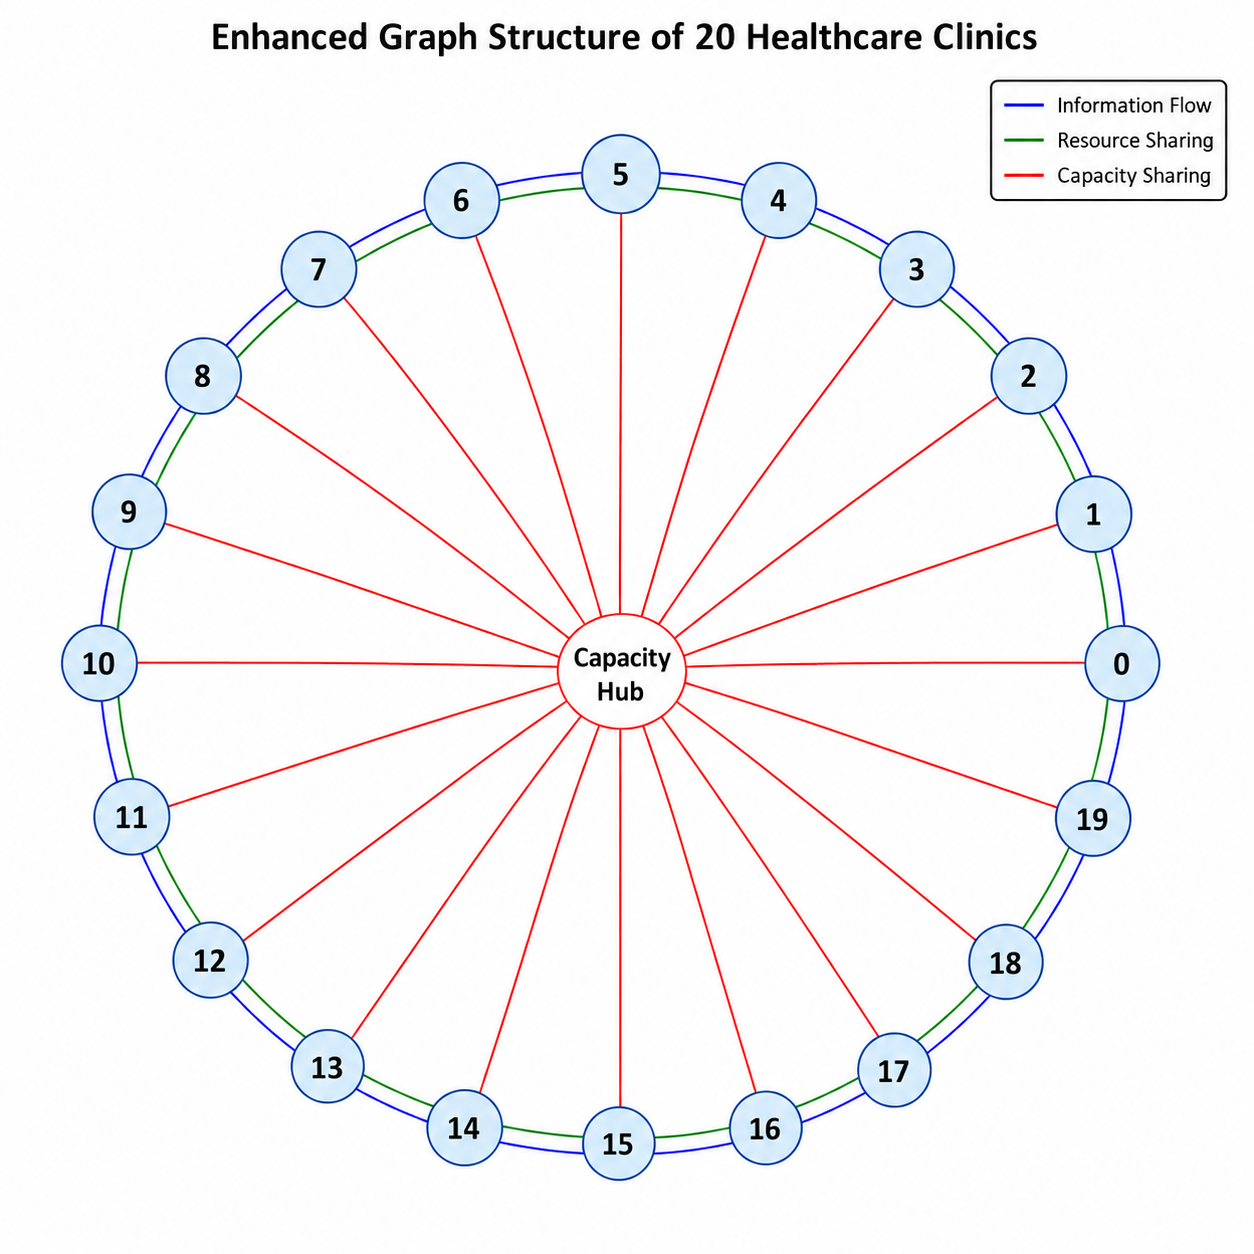
\includegraphics[width=0.78\textwidth]{figures/Figure 2.png}
    \caption{Graph representation of a distributed personalized regenerative medicine manufacturing network with 20 healthcare clinics. Each outer node represents a clinic or manufacturing facility, and the central node represents the shared capacity pool. Blue edges indicate information flow among neighboring clinics, green edges indicate fungible-resource relationships, and red radial edges indicate capacity sharing between each clinic and the central capacity hub. Qualified specimen-logistics links are configured as a constrained subset of inter-clinic relationships and are omitted from this conceptual edge legend. The graph convolutional network encodes local and neighboring state for downstream patient-indexed routing and resource decisions.}
    \label{fig:graph_structure}
\end{figure}

Formally, let $G_t=(V,E_t)$ represent the manufacturing network at epoch $t$, where each node
$v_i\in V$ denotes a facility with state features $x_i^t$ and edge weights $e_{ij}^t$ indicate
logistic or transshipment costs. The GCN encodes local and neighborhood information using a
layer-wise propagation rule:
\begin{equation}
h_i^{(l+1)} = \sigma \Big(W^{(l)} \sum_{j \in \mathcal{N}(i)} \frac{1}{c_{ij}} h_j^{(l)} \Big),
\end{equation}
where $h_i^{(0)} = x_i^t$, $W^{(l)}$ are trainable weights, $\sigma(\cdot)$ is a ReLU activation,
and $c_{ij}$ is a degree-based normalization factor. The resulting embedding
$H_t = \{h_i^{(L)}\}_{i=1}^{N}$ captures the current global state of the network.
\subsection*{Overview of the graph-aware actor--critic workflow (DDPG instantiation)}

Training has two explicit stages. First, common-random-number look-ahead constructs advantage-filtered residual targets relative to MDL-2 and initializes the graph encoder and actor on those targets. Second, DDPG interacts with the simulator, stores feasibility-projected actions and rewards in replay, and updates the critic, actor, and shared encoder while retaining the filtered teacher loss as an actor regularizer. At execution time, the observed node features change with queues, patient condition, inventories, disruptions, and transit pipelines; the configured clinic topology supplies the graph over which the same learned encoder aggregates those dynamic features. The GCN therefore processes a time-varying network state but does not infer a new physical network at every epoch.

This two-stage description is important for attribution. AFR-GCN--DDPG denotes the controller that results from the complete procedure, whereas final-versus-frozen comparisons separately test whether the online DDPG phase adds endpoint value beyond the advantage-filtered initialization.


\subsection*{Initialization}
\begin{itemize}
\item Critic network \( Q(X_t, A_t|\theta_Q) \) initialized with weights \( \theta_Q \).
\item Actor network \( \mu(X_t|\theta_\mu) \) initialized with weights \( \theta_\mu \).
\item GCN initialized with weights \( \omega \) for processing graph states.
\end{itemize}

\subsection*{DDPG Component}
The DDPG agent operates on the GCN-encoded state $H_t$ to generate a bounded residual action
$\Delta A_t=\mu(H_t|\theta_\mu)$. Let $A_t^{\mathrm{anc}}$ denote the action produced by the
transparent look-ahead anchor and let $\rho$ be a vector of decision-group-specific trust-region
scales. The raw proposed action is
\begin{equation}
A_t^{\mathrm{raw}}=A_t^{\mathrm{anc}}+\rho\odot\Delta A_t.
\end{equation}
This residual parameterization preserves the anchor's basic inventory logic while allowing the GCN
policy to adapt patient-indexed specimen routing, replenishment, and fungible resource-sharing decisions to network-wide
patient pressure, geographic connectivity, disruptions, and demand-prior drift. The critic network
$Q(H_t,A_t|\theta_Q)$ estimates expected discounted return, where reward is the negative modeled
cost. The optimization follows the standard DDPG updates:
\begin{align}
y_i &= r_i + \gamma Q'(H_{i+1},\mu'(H_{i+1}|\theta_{\mu'})|\theta_{Q'}),\\
L_Q &= \frac{1}{N}\sum_i (y_i - Q(H_i,A_i|\theta_Q))^2,\\
\nabla_{\theta_\mu} J &= \frac{1}{N}\sum_i \nabla_a Q(H_i,a|\theta_Q)|_{a=\mu(H_i)} 
\nabla_{\theta_\mu} \mu(H_i|\theta_\mu).
\end{align}

\subsection*{Advantage-filtered residual initialization and deployment}
The useful residual corrections in AFR-GCN--DDPG are sparse because the MDL-2 anchor is already
competitive in many states. We therefore initialize the residual actor through
advantage-filtered teacher construction. At a sampled state, we compare a small set of
decision-group residual candidates, including specimen routing and network-resource actions, with the zero-residual
MDL-2 action over a finite look-ahead horizon. Candidate and anchor rollouts use
common random numbers so that their score difference is not dominated by
different demand, deterioration, or disruption realizations. A nonzero target
is retained only when it improves the configured operating-cost and
patient-outcome score; otherwise the target is the zero residual. To keep the
sparse improvement labels from being overwhelmed, improving and zero-residual
examples receive equal total weight. The weighted advantage-filtered data remain in the actor
loss during DDPG fine-tuning rather than being used only as a one-time warm
start.

Deployment uses two independent validation stages. First, checkpoints saved
during training are compared on common validation scenarios. Second, the
selected checkpoint is evaluated over a fixed set of residual trust-region
scales, including zero. The nonzero residual is deployed only when it improves
validation cost without reducing service; otherwise the controller falls back
to MDL-2. This mechanism keeps the deployed controller within the residual
GCN--DDPG family while preventing a poorly generalized correction from
overriding the operational anchor.

\subsection*{Reward function}
The agents optimize the negative of the immediate cost defined in Section~\ref{sec:problem-graph-mdp}. For each epoch $t$, the reward is
\begin{equation}
r_t = -\,c(\mathbf{A}_t;\tilde{\mathbf{X}}_t),
\end{equation}
where $c(\cdot)$ is the extended cost of Equation~\eqref{eq:cost}, comprising the operational base cost $c_{\mathrm{op}}$ (reagent purchase, holding, and shortage; bioreactor holding and shortage; specimen and reagent logistics; and capacity relocation) together with the patient-loss, material-and-product-expiry, and urgency terms. Optimizing this reward therefore requires the agent to trade current operating and logistics cost against the future risk of patient losses and expiry, rather than resource utilization alone.


\begin{algorithm}[p]
\footnotesize
\caption{Graph-aware actor--critic for distributed PRM capacity planning (DDPG instantiation; TD3/SAC/PPO swap the critic target, policy parameterization, or update schedule).}
\label{alg:ddpg_gcn}
\begin{algorithmic}[1]
\Require Anchor policy $\pi_{\mathrm{anc}}$, residual candidates $\mathcal{D}$, look-ahead horizon $L$, discount factor $\gamma$, soft-update rate $\tau$, actor and critic learning rates $\alpha_\mu,\alpha_Q$, exploration scale $\sigma$, minibatch size $N$.
\State Initialize GCN encoder $g_\omega$, actor $\mu(\cdot\mid\theta_\mu)$, critic $Q(\cdot,\cdot\mid\theta_Q)$, target networks $\mu'$ and $Q'$, and replay buffer $\mathcal{R}$.
\State Build weighted teacher data by comparing $\pi_{\mathrm{anc}}(X)+\delta$, $\delta\in\mathcal{D}$, with $\pi_{\mathrm{anc}}(X)$ under common-random-number $L$-step rollouts; use target $\delta^*$ only when it improves the score and zero otherwise.
\State Fit the residual actor to the weighted advantage-filtered targets and retain this loss as an actor regularizer.
\For{each environment step $t$}
    \State Observe raw graph state $X_t$ and compute graph embedding $Z_t=g_\omega(X_t)$.
    \State Select exploratory residual action $A_t=\pi_{\mathrm{anc}}(X_t)+\rho\odot\mu(Z_t\mid\theta_\mu)+\epsilon_t$, where $\epsilon_t\sim\mathcal{N}(0,\sigma^2 I)$.
    \State Project or clip $A_t$ to the feasible set and execute the resulting action $\hat{A}_t$.
    \State Observe cost/reward $r_t$, next state $X_{t+1}$, and store $(X_t,\hat{A}_t,r_t,X_{t+1})$ in $\mathcal{R}$.
    \If{an update is scheduled}
        \State Sample minibatch $(X_i,A_i,r_i,X_{i+1})_{i=1}^{N}$ from $\mathcal{R}$ and compute $Z_i=g_\omega(X_i)$, $Z_{i+1}=g_\omega(X_{i+1})$.
        \State Compute targets $y_i=r_i+\gamma Q'(Z_{i+1},\mu'(Z_{i+1}\mid\theta_{\mu'})\mid\theta_{Q'})$.
        \State Update critic by minimizing $L_Q=N^{-1}\sum_i(y_i-Q(Z_i,A_i\mid\theta_Q))^2$.
        \State Update actor using the deterministic policy gradient plus the weighted advantage-filtered regularizer.
        \State Backpropagate through the GCN encoder and softly update target networks.
    \EndIf
\EndFor
\State Select checkpoint and residual scale on independent validation scenarios; return the calibrated residual policy or the MDL-2 fallback.
\end{algorithmic}
\end{algorithm}

\paragraph{Action decoding and feasibility projection.}
Because the actor network outputs continuous residuals, an additional deterministic decoding and feasibility-projection step is used before actions are executed in the simulation environment. The raw anchor-plus-residual action $A_t^{\mathrm{raw}}$ is first scaled to the admissible range of each decision variable and then clipped to its variable-specific lower and upper bounds. The specimen block expresses signed facility pressure rather than anonymous divisible flow. It is scaled by the maximum route quantity and rounded half away from zero to integer requests; a shared executor then matches opposite requests only across qualified edges and selects specific eligible patient identities. Reagent transshipment, bioreactor relocation, and replenishment are decoded through their corresponding bounds and feasibility rules.

The decoded action is subsequently passed through a repair operator that enforces the operational constraints of the manufacturing network. First, nonnegativity constraints are imposed so that the resulting action cannot remove more reagents, idle bioreactors, or route-eligible waiting specimen lots from a facility than are available at that epoch. Second, replenishment quantities are capped by the maximum purchasable reagent quantity $P_t^n$ and by supplier availability. Third, network conservation is enforced separately for fungible resources and integer specimen lots. A specimen route is legal only for a waiting identity that has not previously moved; each executed donor event has one matched receiver event, and unmatched requests are recorded as blocked rather than repaired by substitution. Finally, all transfer and routing actions are restricted to their configured graph edges. Finished-product return is a deterministic identity-preserving lifecycle transition, not an actor decision.

Equivalently, the executed action can be interpreted as the feasible action $\hat{A}_t$ obtained by projecting the decoded actor output onto the feasible action set $\mathcal{F}(X_t)$:
\begin{equation}
\hat{A}_t = \Pi_{\mathcal{F}(X_t)}\!\left(A_t^{\mathrm{raw}}\right),
\end{equation}
where $\mathcal{F}(X_t)$ is determined by current facility states, patient lifecycle and route history, inventory availability, capacity availability, supplier limits, the autologous identity constraint, and graph connectivity. This projection step improves engineering credibility by ensuring that all actions executed in the simulation correspond to implementable specimen-routing, capacity, replenishment, and transshipment decisions.


Each stability-oriented backbone reuses this encoder and projection layer unchanged and alters only the reinforcement-learning update. TD3 replaces the single critic with clipped double-$Q$ targets, delays actor updates, and adds target-policy smoothing; SAC replaces the deterministic actor with an entropy-regularized stochastic policy and a soft value target; and PPO replaces off-policy replay with on-policy rollouts optimized under a clipped surrogate objective. In all cases the actor and critic operate on the GCN embedding $Z_t$ rather than on the flat state, and the executed action is the feasibility-projected $\hat{A}_t$.

\subsection*{Summary}

The proposed method is therefore a residual GCN--DDPG controller: a GCN encoder supplies a permutation-equivariant, network-aware state representation; a deterministic actor learns bounded corrections to a transparent look-ahead anchor; and a feasibility-projection layer guarantees that every executed action respects inventory, capacity, supplier, patient identity, route history, and connectivity constraints. The routing-primary architecture comparison holds specimen-routing availability, the anchor, residual action space, advantage-filtered teacher protocol, projection, training budget, and evaluation seeds fixed between GCN and parameter-matched flat encoders. The earlier backbone comparison instead holds the graph encoder fixed while replacing DDPG with TD3. Residual SAC and PPO are secondary family extensions because their stochastic residual distributions and likelihood calculations require additional matched implementation work. These variants test backbone robustness without redefining them as separate proposed methods.
\section{Computational Experiments}
\label{sec:experiments}
\label{sec:casestudies}

This section reports three empirical stages designed to separate anchor improvement, graph representation, and online reinforcement-learning attribution. The first stage calibrates patient-condition dynamics and evaluates replenishment residuals under demand-prior drift. The second expands the action space to geographically structured reagent and idle-capacity transfers and compares the graph policy with a parameter-matched flat policy. The third holds the pretrained graph controller fixed while testing whether conservative online TD3 updates add value beyond frozen pretraining. The experiments compare the learned graph-aware correction policy with its heuristic anchor, other heuristic and look-ahead policies, flat-state residual policies, and graph-aware backbone variants under the same simulation environment.
\subsection{Objective}
The objective of this study is to compare the proposed residual GCN--DDPG framework with traditional heuristic methods, its MDL-2 anchor, flat-state residual DDPG, and stability-oriented graph-aware actor--critic variants in distributed manufacturing.

\subsection{Methodology}

\subsubsection{Benchmarking Setup}
The final benchmark is organized as a hierarchy of matched comparisons rather
than a single undifferentiated algorithm ranking (Table~\ref{tab:final_benchmark}).
The first comparison tests whether reinforcement learning improves the MDL-2
anchor. The second isolates the graph representation by replacing the GCN with
a flat MLP while keeping the entire residual-learning recipe fixed. The third
tests whether the result is specific to DDPG by repeating the residual
comparison with TD3. Online rollout shields and the supervised GCN shield
selector are reported separately because the former uses additional simulation
at decision time and the latter is not an RL policy. Pure end-to-end RL and the
stochastic SAC/PPO family are reported as secondary comparators rather than
being allowed to substitute for these mandatory tests.

The heuristic baselines are:
\begin{itemize}
\item \textbf{MYO (Myopic):} This heuristic minimizes single-period cost without considering future demand.
\item \textbf{MDL-1 (One-period Mean Demand Lookahead):} MDL-1 extends the planning horizon to one lookahead period using deterministic state transitions based on mean demand.
\item \textbf{MDL-2 (Two-period Mean Demand Lookahead):} MDL-2 extends the planning horizon to two lookahead periods using deterministic state transitions based on mean demand.
\item \textbf{ISO (Isolated Regional Facilities):} ISO assumes no resource sharing between facilities and focuses only on local replenishment decisions.
\item \textbf{F-MYO (Forecast Myopic):} F-MYO augments current-period network balancing with the demand forecast available at the decision epoch.
\item \textbf{uMYO and pMYO (Patient-aware myopic policies):} uMYO adds urgency-based replenishment and capacity surges, while pMYO uses a bounded patient-risk workload uplift. These controls prevent the proposed method from being compared only with condition-blind heuristics.
\end{itemize}

The learning-based comparisons are:
\begin{itemize}
\item \textbf{MLP residual DDPG / flat-state residual DDPG:} This baseline uses the same MDL-2 anchor, residual action space, DDPG actor--critic structure, training budget, and feasibility projection as the proposed method, but removes the GCN encoder. Instead, all facility-level states are concatenated into a flat vector and passed directly into multilayer perceptron actor and critic networks. This baseline is designed to answer whether performance improvements come from reinforcement learning alone or from explicitly encoding graph-structured inter-facility dependencies.
\item \textbf{Residual GCN--TD3 and matched flat residual TD3:} These policies keep the anchor, advantage-filtered supervision, action constraints, training data, and evaluation streams fixed while replacing the DDPG update with TD3. They test whether twin critics, delayed actor updates, and target smoothing improve stability.
\item \textbf{Pure GCN and flat actor--critic policies:} From-scratch DDPG and TD3 quantify the benefit of anchoring; SAC and PPO provide secondary off-policy stochastic and on-policy comparisons. Residual SAC/PPO are included only after their residual-space probability calculations and matched flat variants pass the same validation protocol.
\end{itemize}

\begin{table}[htbp]
\centering
\footnotesize
\caption{Final comparison hierarchy for the proposed controller.}
\label{tab:final_benchmark}
\setlength{\tabcolsep}{3pt}
\renewcommand{\arraystretch}{1.0}
\begin{tabularx}{\textwidth}{p{0.17\textwidth} p{0.37\textwidth} X}
\toprule
Comparison layer & Required policies & Question answered \\
\midrule
Anchor improvement & AFR-GCN--DDPG versus MDL-2 & Does the learned correction improve the strong policy from which it starts? \\
Strong heuristics & ISO, MYO, F-MYO, uMYO, pMYO, MDL-1, and MDL-2 & Is the controller competitive with sharing, forecast-aware, patient-aware, and look-ahead rules? \\
Representation ablation & AFR-GCN--DDPG versus matched AFR-flat-DDPG & Is any gain attributable to graph representation rather than residual learning alone? \\
Backbone robustness & Residual GCN--DDPG versus residual GCN--TD3, each with a matched flat counterpart & Does the result persist when the deterministic actor--critic backbone changes? \\
Anchor ablation & Residual versus pure GCN/flat DDPG and TD3 & Does the heuristic anchor improve sample efficiency, stability, and final performance? \\
Deployment reference & MDL-2/pMYO rollout shields and supervised GCN shield selector & How does policy quality trade off against online simulation cost, and can RL outperform non-RL distillation? \\
Secondary family & GCN/flat SAC and PPO; residual forms after matched implementation & Is the conclusion robust to stochastic off-policy and on-policy learning? \\
Graph mechanism & Full graph, no/shuffled edges, and geographic-edge ablations & Does the policy use topology rather than merely additional parameters? \\
\bottomrule
\end{tabularx}
\end{table}

In addition, graph ablation experiments are planned to evaluate the role of different edge types. Specifically, we consider removing capacity-sharing edges and removing resource-sharing edges to assess whether these relational structures contribute to policy performance under disruption and demand uncertainty.

All methods receive the same decision-time observations and are evaluated on
identical paired random-number streams. In demand-prior-drift experiments,
heuristics receive the same misspecified demand prior available to the
controller and no method receives the realized future demand rates. Learned
policies use the same training-scenario distribution, environment-interaction
budget, checkpoint-selection budget, and held-out evaluation seeds within each
matched comparison. Online decision time and the number of simulator rollouts
are reported separately for rollout-based methods. This prevents a performance
difference from being created by unequal forecasts, simulator access,
evaluation noise, or hidden online computation.

\subsubsection{Performance Metrics}

We evaluate each method using both objective-based and
engineering-relevant performance metrics. The primary metric is the average
total weighted objective $J_{\mathrm{tot}}$ in
Equation~\eqref{eq:episode-objective}. It includes the complete operating-cost
group (reagent purchase, holding, and shortage; bioreactor holding and
shortage; and reagent and capacity transfer) and the patient-related penalty
group (patient loss, material or therapy expiry, and urgency). The percentage
improvement reported in headline comparisons always uses the anchor's complete
$J_{\mathrm{tot}}$ as the denominator, as in
Equation~\eqref{eq:relative-total-improvement}; we do not remove large
components after observing the result.

Because a weighted total can be dominated by patient-loss or capacity-shortage
penalties, every formal comparison also reports the absolute paired difference
and an additive cost decomposition. Component-specific percentages are
secondary mechanism measures: they reveal whether a policy saves purchase,
holding, shortage, transfer, or patient-penalty cost, but do not replace the
primary total-objective comparison. When an oracle or other defensible
lower-cost reference is evaluated, we also report the headroom-capture measure
in Equation~\eqref{eq:headroom-captured}. To strengthen the application
relevance of the experiments, we track the following secondary metrics:
\begin{itemize}
    \item \textbf{Cost decomposition:} operating/base cost and its reagent, bioreactor, and transfer components, together with patient-loss, expiry, and urgency penalties.
    \item \textbf{Completion service level:} the fraction of eligible patient demand completed within the planning horizon.
    \item \textbf{Patient loss and manufacturing-period ineligibility:} the number of patients who become ineligible or expire before treatment and the fraction who become ineligible after manufacturing begins.
    \item \textbf{Average waiting time / fulfillment delay:} the average number of epochs that patient specimens wait before manufacturing begins.
    \item \textbf{Reagent shortage frequency:} the frequency with which manufacturing is delayed because insufficient reagents are available.
    \item \textbf{Bioreactor utilization:} the fraction of available bioreactor capacity used for production across facilities.
    \item \textbf{Routing, transshipment, and relocation activity:} patient-indexed specimen route count, distance, transit time, route cost, and blocked requests, together with reagent movements and idle-bioreactor relocations. These are mechanism diagnostics rather than evidence that routing is itself a contribution.
    \item \textbf{Inference time:} the computational time required for a trained policy or heuristic to generate one epoch-level decision.
\end{itemize}

These metrics are included because the objective of PRM capacity planning is
not only to reduce a modeled weighted objective, but also to support timely
patient-specific manufacturing, effective resource utilization, and reliable
system performance under demand and supply uncertainty. Cost-weight
sensitivity is therefore required before translating an objective difference
into an economic claim.

\subsubsection{Heuristic Implementations}
We provide brief descriptions of the heuristic methods implemented:
\begin{itemize}
    \item \textbf{MYO (Myopic):} MYO focuses on minimizing costs within the current period without considering future consequences.
    \item \textbf{MDL-1 and MDL-2:} These methods extend the planning horizon to one and two lookahead periods, respectively, using deterministic state transitions based on mean demand.
    \item \textbf{ISO (Isolated Regional Facilities):} ISO assumes no sharing of resources between manufacturing facilities and primarily concentrates on reagent replenishment.
\end{itemize}

\subsubsection{Implementation and statistical protocol}
The models are implemented in Python using PyTorch, and all experiment
parameters, training seeds, checkpoint candidates, deployment scales, and
evaluation streams are stored in configuration files. Within a matched
comparison, the graph and flat policies receive the same state variables,
anchor actions, teacher targets, environment interactions, validation budget,
and common-random-number (CRN) holdout episodes. The graph policy replaces the
flat encoder with message passing over the clinic graph; the remaining
actor--critic and deployment components are held fixed or parameter matched.

\paragraph{Routing-primary hyperparameter development}
The routing-primary DDPG settings were obtained through sequential,
development-only sensitivity screens rather than an exhaustive automated HPO
search. The screens first bounded the residual correction and then varied the
online update schedule, actor learning rate, exploration noise, imitation and
frozen-reference regularization, and deployment gate. Mechanism-development
screens separately examined integer-lot straight-through specimen actions,
anchor-relative rewards, return horizon, and evidence required to release the
frozen-pretraining reference. Table~\ref{tab:routing_hyperparameters}
summarizes the principal ranges and the current candidate. All screens used
development seeds and CRN streams; none is included in a confirmatory estimate.

\begin{table}[htbp]
\centering
\footnotesize
\caption{Routing-primary DDPG development screens. The selected values define
the current candidate but are not themselves confirmatory results.}
\label{tab:routing_hyperparameters}
\setlength{\tabcolsep}{3pt}
\renewcommand{\arraystretch}{1.05}
\begin{tabularx}{\textwidth}{
  >{\raggedright\arraybackslash}p{0.26\textwidth}
  >{\raggedright\arraybackslash}p{0.41\textwidth}
  >{\raggedright\arraybackslash}X}
\toprule
Component & Development values or variants & Selected value \\
\midrule
Residual deployment magnitude & Anchor-only; 0.10, 0.25, and 0.50 & 0.10 for specimen transfer \\
Environment update frequency & Every 1 or 4 simulator steps & 1 \\
Actor update frequency & Every 2, 4, or 8 critic updates & 2 \\
Online actor learning rate & $1\times10^{-5}$ or $3\times10^{-5}$ & $1\times10^{-5}$ \\
OU exploration standard deviation & 0.005, 0.02, or 0.05 & 0.005 \\
Imitation/reference regularization & Imitation 1 or 2; reference 0, 250, or 500 & 1 and 500, respectively \\
Pretraining/critic warm start & Short smoke or 300 epochs; 0 or 500 critic updates & 300 epochs and 500 updates \\
Online return evidence & Immediate or four-step anchor-relative return; unfiltered, positive, or dual confirmation & Four-step dual confirmation \\
Material improvement threshold & Zero or one patient-loss-equivalent scaled cost & 0.0005 \\
Deployment gate & Fixed development validation grid with anchor fallback & 0.575 \\
\bottomrule
\end{tabularx}
\end{table}

The selected candidate uses batch size 64, critic learning rate
$3\times10^{-4}$, integer specimen-lot execution with a straight-through actor
gradient, and specimen-only residual corrections; reagent, capacity, and
replenishment residual groups remain zero in this screen. The most informative
warning against single-seed selection came from the update-frequency study:
the frequency-4 candidate passed its seed-0 screen but did not generalize in
the subsequent three-seed confirmation. Seed 0 and the earlier routing seeds
1--2 are therefore treated as development evidence, not untouched
confirmation seeds.

The replenishment-residual DDPG and TD3 confirmation uses 300 training episodes
for each of five seeds, checkpoint candidates between episodes 50 and 300, and
100 independent paired holdout replications per seed. Reported confidence
intervals use a two-level bootstrap over training seeds and paired evaluation
replications. The regional network-action experiment uses three independently
initialized graph and flat policies, 30 paired validation episodes, and 100
previously unseen paired holdout replications per seed. Because its selected
checkpoint is dominated by advantage-filtered teacher distillation, that
experiment is interpreted as graph-policy evidence rather than as independent
evidence for online DDPG updates.

The conservative online-TD3 screen starts from the corresponding frozen
pretrained graph and flat checkpoints and runs 100 online episodes for seeds
0, 1, and 2. Each run completed 5,200 update calls, including 5,073 critic
updates and 2,286 delayed actor updates. Final and frozen checkpoints are
evaluated with identical CRN keys, using 20 validation and 100 holdout
replications per seed for the final policies and 5 validation and the same 100
holdout replications per seed for the frozen controls. This campaign was run
on an NVIDIA RTX 4090 GPU; all optimization diagnostics were finite, and no
CPU fallback occurred. These experiment-specific budgets replace the earlier
generic one-million-step description and make the reported results traceable
to the executed configurations.

The routing-primary campaign is prospectively separated from those earlier
no-routing results. It holds patient-indexed specimen routing enabled for every
primary policy and compares GCN residual DDPG, a parameter-matched flat
residual DDPG controller, and the MDL-2 routing anchor. One fresh
routing-enabled teacher is shared across the learned architectures. After the
development screens are frozen, confirmatory training uses five untouched
seeds (10--14) for each learned architecture. Every run first
receives 100 episodes, or approximately 5,200 online transitions, with complete
state saved every five episodes. Prespecified development learning curves at
episodes 25, 50, 75, and 100 determine one global budget decision before the
final holdout is opened: if either architecture has not plateaued, all ten runs
are extended to 200 episodes. Extension to the common maximum of 300 is allowed
only if the 100--200 curves show continuing multi-seed improvement without
clinical-guardrail deterioration. A method- or seed-specific extension is not
permitted.

Final and frozen-pretraining checkpoints are evaluated on four routing
scenarios with at least 100 paired CRN replications per training seed;
additional evaluation replication may narrow uncertainty without changing the
trained policies. Lead-zero specimen transit and one-epoch product return are
prespecified sensitivities. The primary attribution is GCN versus matched
flat, GCN versus MDL-2, and final versus frozen pretraining. No-routing is
retained only for deterministic mechanics regression or a separately approved
supplementary ablation, not as a default formal training arm. Development
screens are reported as tuning evidence only, and no routing-primary headline
claim is made until the untouched-seed outputs pass the locked gates.
\subsection{distributed manufacturing simulation}
% Algorithm for state normalization with changed variables
\begin{algorithm}
\caption{State normalization}
\begin{algorithmic}[1]
\Require State variables: $s_t^n$, $r_t^n$, $b_t^n$, and $p_t^n$ \\
         Maximal values of the state variables for all facilities: $M_s$, $M_r$, $M_b$, and $M_p$
\Ensure Normalized state variables: $\hat{s}_t^n$, $\hat{r}_t^n$, $\hat{b}_t^n$, $\hat{p}_t^n$

\For{$n = 1$ to $N$}
    \State $\hat{s}_t^n = s_t^n / M_s$
    \State $\hat{r}_t^n = r_t^n / M_r$
    \State $\hat{b}_t^n = b_t^n / M_b$
    \State $\hat{p}_t^n = p_t^n / M_p$
\EndFor
\end{algorithmic}
\end{algorithm}

To evaluate the proposed method, we now construct a simulation environment of a decentralized manufacturing system consisting of $N=20$ manufacturing facilities and its dedicated reagent supplier. Each PRM product requires $T=3$ epochs of manufacturing time, and the considered finite problem horizon contains $\Gamma=52$ decision epochs. For every epoch $t$, there will be $d_{t}^{n}$ new demand for facility $n$. The demand arrival process for facility $n$ follows a Poisson distribution $\text{Poisson}\left(\lambda_{n}\right)$. The supplier disruption follows independent Bernoulli processes $\text{Ber}\left(\zeta_{n}\right)$, i.e., the facility $n$ has a probability $\zeta_{n}$ to have supplier disruption and could not purchase any reagent for the epoch. This simulation can be further adjusted to reflect any real situation, e.g., supply disruption and demand uncertainty, that may be encountered. Such flexibility in using the simulation system will be demonstrated in Section 5.4 when we compare GCN-DDPG with other methods.

Patient-condition parameters are calibrated before policy comparison. The
nominal scenario uses $\lambda_H=0.0013$, $\lambda_F=0.0156$, Weibull shape
$\kappa=1.5$ and scale $\theta=4$, post-deterioration acceleration $\rho=3$,
eligibility threshold $\epsilon=0.80$, and waiting-time pressure
$0.0013\alpha^2$. We selected these values from a fixed-seed sweep whose
pre-specified target was a 10--15\% \emph{patient ineligibility during
manufacturing} rate over the three-week process. This outcome is not labeled a
technical manufacturing failure: it records a patient who becomes clinically
ineligible after production begins, whereas a process or release-specification
failure would be a separate stochastic event. The target is consistent with the
order of magnitude of pre-infusion attrition reported for autologous CAR-T
pathways~\cite{AyalaCeja2024CARTManufacturing} and with a 5\% weekly
eligibility-transition benchmark, which gives
$1-(1-0.05)^3=14.26\%$ over three weeks.

The patient-facing weights are
$\omega_{\mathrm{lost}}=500{,}000$,
$\omega_{\mathrm{exp}}=100{,}000$, and
$\omega_{\mathrm{urg}}=25{,}000$. The earlier exploratory values
$(50{,}000,40{,}000,5{,}000)$ made one-time patient loss cheaper than even one
period of combined reagent and bioreactor shortage, so a policy could lower its
objective when a patient left the system. The calibrated ordering removes this
directional inconsistency and is held fixed for all policy comparisons.

The epoch is assumed to occur weekly. Reagent and idle-bioreactor transfers
enter an in-transit pipeline and arrive after one, two, or three epochs,
according to whether the geographic distance is at most 500 miles, between 500
and 1,500 miles, or above 1,500 miles. In the routing-primary campaign, an
intact waiting specimen may take one direct qualified route. The main setting
uses one transit epoch and immediate modeled return of finished product to the
collection facility; zero-epoch specimen transit and one-epoch product return
are sensitivities. The previously reported case studies set $w_t^n=0$ and are
therefore not routing-effect experiments. After demand and any due transfers
or routes have arrived, the next observed state is
$\mathbf{x}_{t+1}^{n}=\left(s_{t+1}^{n}, r_{t+1}^{n}, \mathbf{b}^{n},
P_{t+1}\right)$ for facility $n=1, \ldots, N$, according to Equation (1). The
state variables are updated by the following rules:

\begin{align*}
s_{t+1}^{n}&=s_{t}^{n}-m_{t}^{n}+d_{t}^{n}+w_{t}^{n} \\
r_{t+1}^{n}&=r_{t}^{n}-m_{t}^{n}+e_{t}^{n}+p_{t}^{n} \\
b_{t+1}^{n, \tau}&= \begin{cases}
b_{t}^{n, 0}-m_{t}^{n}+b_{t}^{n, 1}+q_{t}^{n} & \text{if } \tau=0 \\
b_{t}^{n, \tau+1} & \text{if } 1 \leq \tau \leq T-2 \\
m_{t}^{n} & \text{if } \tau=T-1
\end{cases}
\end{align*}

where $m_{t}^{n}=\min \left(s_{t}^{n}, b_{t}^{n, 0}, r_{t}^{n}\right)$ is the number of products that begin manufacturing at epoch $t$, $d_{t}^{n}$ is the demand arriving at facility $n$ in epoch $t$, and $P_{t+1}$ follows an exogenous Markov chain from $P_{t}$. The operating component of the single-period objective can be decomposed as

\begin{align*}
c_{\mathrm{op}}\left(\mathbf{A}_{t};\mathbf{X}_{t}\right)
&=\sum_{n=1}^{N} C_{\mathrm{op},t}^{n},\\
C_{\mathrm{op},t}^{n}
&=C_{\text{Reg},t}^{n}+C_{\text{Bio},t}^{n}+C_{\text{Tran},t}^{n}.
\end{align*}

The meanings of $C_{\text{Reg},t}^{n}$, $C_{\text{Bio},t}^{n}$, and
$C_{\text{Tran},t}^{n}$ are summarized below. These terms constitute only
$c_{\mathrm{op}}$; the patient-related terms in Equation~\eqref{eq:cost} must
also be included to obtain the total weighted objective.

\begin{itemize}
  \item $C_{\text{Reg}, t}^{n} = c_{R} p_{t}^{n} + h_{R}\left(r_{t+1}^{n}-s_{t+1}^{n}\right)^{+} + p_{R}\left(s_{t+1}^{n}-r_{t+1}^{n}\right)^{+}$ is the cost related to reagent at epoch $t$, including the reagent replenishment cost $c_{R} p_{t}^{n}$, the reagent overstock holding cost $h_{R}\left(r_{t+1}^{n}-s_{t+1}^{n}\right)^{+}$, and the reagent understock penalty $p_{R}\left(s_{t+1}^{n}-r_{t+1}^{n}\right)^{+}$;
  \item $C_{\text{Bio}, t}^{n} = h_{B}\left(b_{t+1}^{n, 0}-s_{t+1}^{n}\right)^{+} + p_{B}\left(s_{t+1}^{n}-b_{t+1}^{n, 0}\right)^{+}$ is the cost related to bioreactor at epoch $t$, including the bioreactor overstock holding cost $h_{B}\left(b_{t+1}^{n, 0}-s_{t+1}^{n}\right)^{+}$, and the bioreactor understock penalty $p_{B}\left(s_{t+1}^{n}-b_{t+1}^{n, 0}\right)^{+}$;
  \item $C_{\text{Tran}, t}^{n} = K_{R}\left|e_{t}^{n}\right| + K_{B}\left|q_{t}^{n}\right| + K_{S}\left|w_{t}^{n}\right|$ is the logistics-cost expression. The routing-primary campaign includes the patient-indexed specimen term; it vanishes only in the earlier no-routing case studies.
\end{itemize}

\begin{table}[ht]
\centering
\caption{Modeled cost coefficients used in the calibrated experiments. Values are weighted-objective units and are held fixed across policies. Transfer coefficients are base values before the geographic distance and travel-time surcharge. Patient-related coefficients are penalty or shadow-value parameters rather than observed cash expenditures.}
\label{tab:cost_coefficients}
\begin{tabular}{lrl}
\hline
Component & Coefficient & Interpretation \\
\hline
Reagent purchase, $c_R$ & $42{,}174.0$ & per purchased unit \\
Reagent holding, $h_R$ & $113.5$ & per excess unit-period \\
Reagent shortage, $p_R$ & $86{,}504.5$ & per shortage unit-period \\
Bioreactor holding, $h_B$ & $14.4$ & per idle unit-period \\
Bioreactor shortage, $p_B$ & $50{,}273.6$ & per shortage unit-period \\
Reagent transfer, $K_R$ & $200.0$ & per transferred unit, before surcharge \\
Capacity transfer, $K_B$ & $500.0$ & per relocated unit, before surcharge \\
Patient loss, $\omega_{\mathrm{lost}}$ & $500{,}000$ & per lost patient \\
Expiry, $\omega_{\mathrm{exp}}$ & $100{,}000$ & per wasted material or therapy unit \\
Urgency, $\omega_{\mathrm{urg}}$ & $25{,}000$ & per at-risk unserved patient-period \\
\hline
\end{tabular}
\end{table}

\subsection{Case Study 1: Interconnected Clinic Network Analysis}
\label{subsec:casestudy1}
This case study holds the demand prior equal to the arrival distribution and
varies the supplier disruption rate over $0.05$, $0.30$, and $0.60$. Its purpose
is to measure the value of graph-aware coordination when the deterministic
heuristics are not disadvantaged by demand misspecification. The final matched
multi-seed campaign for these three regimes is still pending; consequently, we
do not report numerical disruption-effect claims in the present draft. This
case study will use the same five training seeds, paired Monte Carlo evaluation,
checkpoint selection, and two-level bootstrap protocol as Case Study~2.

\subsection{Case Study 2: Adaptability to Non-Stationary Demand}
\label{subsec:casestudy2}
This case study evaluates the main robustness hypothesis under patient-condition
and geographic network dynamics. The 20 clinics are partitioned into four
five-clinic demand groups. MDL-2 plans with Poisson prior rates
$[7.5,3.2,6.0,3.5]$, whereas the simulator generates arrivals using true rates
$[10.5,3.52,7.5,3.15]$. The environment also includes patient deterioration,
expiry, clustered demand shocks, regional supplier disruptions, and
distance-dependent transfer lead times. During training, demand rates are
randomized between $0.8$ and $1.5$ of the scenario rates and forecast error
between $0$ and $0.35$; evaluation is fixed to the scenario above.

Before retraining learned policies, we evaluated ISO and MDL-2 with 100 paired
Monte Carlo replications to verify that the calibrated patient process and
objective produce the intended clinical range. Table~\ref{tab:demand_drift_results}
reports this calibration pilot and the subsequent matched learned-policy
screen. Learned-policy results produced before the complete patient lifecycle
and objective calibration are not comparable and are therefore retired rather
than carried forward into this experiment.

\begin{table}[ht]
\centering
\caption{Calibrated demand-prior-drift results. ISO and MDL-2 use the initial 100-replication calibration stream; learned-policy and matched heuristic rows aggregate 100 paired replications for each of three training seeds. Objective values are the total modeled weighted objective in billions of cost units, not realized accounting expenditure. Lower objective, patient loss, and manufacturing-period ineligibility are better; higher completion service and eligibility are better.}
\label{tab:demand_drift_results}
\resizebox{\textwidth}{!}{%
\begin{tabular}{lrrrrr}
\hline
Method & Objective ($10^9$ units) & Completion & Eligibility & Lost & Mfg. inelig. \\
\hline
Initial ISO calibration & 3.990456 & 0.337612 & 0.377537 & 4021.92 & 0.146398 \\
Initial MDL-2 calibration & 3.895694 & 0.371948 & 0.421024 & 3698.87 & 0.121364 \\
\hline
AFR-Flat-DDPG & 3.927584 & 0.370359 & 0.507030 & 3730.36 & 0.122223 \\
AFR-GCN-DDPG & 3.927594 & 0.370359 & 0.507030 & 3730.35 & 0.122223 \\
AFR-GCN-TD3 & 3.927628 & 0.370358 & 0.507030 & 3730.36 & 0.122223 \\
MDL-2 & 3.927620 & 0.370359 & 0.507030 & 3730.36 & 0.122223 \\
ISO & 4.011547 & 0.337521 & 0.460044 & 4043.10 & 0.146468 \\
pMYO & 4.180485 & 0.343311 & 0.496776 & 3894.09 & 0.133332 \\
MYO & 4.194549 & 0.342889 & 0.496586 & 3897.01 & 0.133582 \\
\hline
\end{tabular}
}
\end{table}

Both heuristics fall inside the pre-specified clinical calibration band:
manufacturing-period patient ineligibility is 14.64\% for ISO and 12.14\% for
MDL-2. MDL-2 reduces the mean total weighted objective by 94.76 million
modeled cost units (2.37\%) relative to ISO; the paired 95\% interval for
MDL-2 minus ISO is $[-108.81,-80.71]$ million cost units, and MDL-2 has a
lower objective in 92 of 100 paired replications. It also loses 323.05 fewer
patients on average, discards 49.40 fewer in-process therapies, and raises
completion service by 0.03434.

The calibrated learned-policy screen used 100 training episodes and three
training seeds. AFR-GCN--DDPG selected and deployed a nonzero residual in all
three seeds; AFR-GCN--TD3 and AFR-Flat-DDPG each returned to MDL-2 in one seed.
AFR-GCN--DDPG reduced the mean total weighted objective relative to MDL-2 by
only 26,519 modeled cost units ($0.000675\%$), with a two-level bootstrap
95\% interval of $[-89{,}588,40{,}330]$ cost units. Its mean objective was
9,460 cost units higher than the matched flat residual policy, with interval
$[-7{,}951,24{,}621]$. Completion service and patient loss were effectively
unchanged. Thus the screen
demonstrates safeguard-compatible parity with a strong anchor, but it does not
support either a material RL improvement or a graph-representation advantage.
The accepted correction primarily substitutes additional reagent purchase and
holding cost for lower reagent shortage cost. Because this residual changes
replenishment only, the next matched experiment expands the bounded correction
to distance-aware reagent and idle-bioreactor transfers, where geographic
message passing can affect the decision.

The small headline percentage in this screen is intentionally computed against
the complete weighted objective rather than a narrower, post hoc denominator.
Patient-related penalties and capacity-shortage penalties can dominate that
total, while a replenishment-only residual directly changes only a subset of
the operating components. We therefore interpret $0.000675\%$ as statistical
parity rather than as a material economic saving. Subsequent network-residual
comparisons report the total-objective change together with operating,
bioreactor-shortage, transfer, and patient-penalty decompositions so that
denominator dilution and the mechanism of any improvement remain visible.

\subsubsection{Formal five-seed demand-prior-drift confirmation}

The formal replenishment-residual comparison increased the training budget to
300 episodes and used five independent training seeds. Each selected
checkpoint was evaluated on 100 paired holdout replications, yielding 500
paired outcomes per method. Table~\ref{tab:formal_drift_levels} reports the
mean outcomes, and Table~\ref{tab:formal_drift_pairs} reports paired
differences. The learned-policy values in these tables supersede the
100-episode diagnostic screen in Table~\ref{tab:demand_drift_results}.

\begin{table}[htbp]
\centering
\caption{Five-seed demand-prior-drift confirmation. Objective values are the total modeled weighted objective in billions of units. Each row aggregates 100 paired holdout replications for each of five training seeds.}
\label{tab:formal_drift_levels}
\resizebox{\textwidth}{!}{%
\begin{tabular}{lrrrrrr}
\hline
Method & Objective ($10^9$ units) & Completion & Eligibility & Waiting & Lost & At-risk unserved \\
\hline
MDL-2 & 1.268257 & 0.429982 & 0.530313 & 3.052625 & 3665.59 & 5206.41 \\
AFR-Flat-DDPG & 1.268089 & 0.430320 & 0.530523 & 3.052012 & 3663.28 & 5203.86 \\
AFR-GCN--DDPG & \textbf{1.268049} & \textbf{0.430321} & \textbf{0.530524} & \textbf{3.052012} & \textbf{3663.27} & \textbf{5203.86} \\
AFR-GCN--TD3 & 1.268241 & 0.430317 & 0.530523 & 3.052019 & 3663.30 & 5203.88 \\
\hline
\end{tabular}
}
\end{table}

\begin{table}[htbp]
\centering
\caption{Paired five-seed demand-prior-drift comparisons. Differences are candidate minus baseline, so a negative objective difference favors the first method. Confidence intervals use the two-level bootstrap over training seeds and paired replications.}
\label{tab:formal_drift_pairs}
\resizebox{\textwidth}{!}{%
\begin{tabular}{lrrrr}
\hline
Comparison & $\Delta J_{\mathrm{tot}}$ (units) & Relative gap & Paired 95\% CI & Wins / 500 \\
\hline
AFR-GCN--DDPG vs.\ MDL-2 & $-207{,}485$ & $-0.016360\%$ & $[-332{,}641,-91{,}367]$ & 323 \\
AFR-Flat-DDPG vs.\ MDL-2 & $-167{,}610$ & $-0.013216\%$ & $[-286{,}899,-46{,}230]$ & 319 \\
AFR-GCN--DDPG vs.\ AFR-Flat-DDPG & $-39{,}876$ & $-0.003145\%$ & $[-89{,}702,14{,}025]$ & 285 \\
AFR-GCN--TD3 vs.\ MDL-2 & $-15{,}823$ & $-0.001248\%$ & $[-142{,}607,99{,}437]$ & 268 \\
AFR-GCN--DDPG vs.\ AFR-GCN--TD3 & $-191{,}662$ & $-0.015112\%$ & $[-234{,}659,-148{,}401]$ & 377 \\
\hline
\end{tabular}
}
\end{table}

AFR-GCN--DDPG improves on MDL-2 in every training-seed mean and has a
two-level confidence interval fully below zero. Completion service increases
by 0.000340, eligibility by 0.000211, average waiting time falls by 0.000612,
patients lost fall by 2.32, and at-risk unserved patients fall by 2.55. This
supports a statistically stable anchor improvement under demand-prior drift,
but not a large economic effect. The matched flat policy also improves on
MDL-2, and the direct graph-versus-flat interval includes zero. Replenishment
residual learning is therefore supported in this scenario, whereas an
independent graph-representation advantage is not.

The matched TD3 policy preserves the patient-facing improvements but has a
cost interval crossing zero. DDPG is lower cost than TD3 in all five
training-seed means, and their paired interval is fully below zero. This
comparison supports DDPG as the canonical backbone for the proposed
replenishment-residual controller; it is not a claim that DDPG generally
dominates TD3 outside this residual-learning design.

\subsection{Case Study 3: Graph Attribution Under Regional Non-Stationarity}
\label{subsec:casestudy3}

This earlier no-routing case study combines patient-condition dynamics, clinic geography,
distance-based transfer delays, regional demand heterogeneity, and demand
regime changes. Unlike the replenishment-only experiment, the network residual
contains a node head for signed replenishment corrections and edge heads for
reagent and idle-bioreactor transfer corrections. Edge flows are projected to
preserve resource conservation and feasibility, while patient-indexed specimen
routing is disabled by that historical protocol. This action space gives graph message passing a direct route to
affect geographically structured decisions.

\subsubsection{Network AFR-GCN--DDPG under an abrupt regional shift}

The abrupt-shift policy uses transfer-focused advantage-filtered targets and a
fixed deployment scale selected on 30 paired validation episodes. Three
independently initialized graph policies and parameter-matched flat policies
were then evaluated on the same 100 previously unseen paired holdout
replications per seed. The graph and flat models contain 524,775 and 528,404
trainable parameters, respectively, so the comparison does not give the graph
policy a parameter-count advantage.

\begin{table}[htbp]
\centering
\caption{Three-seed abrupt-regional-shift comparisons. Objective differences are in millions of modeled weighted-objective units. Each comparison contains 300 paired holdout outcomes.}
\label{tab:regional_network_pairs}
\resizebox{\textwidth}{!}{%
\begin{tabular}{lrrrrr}
\hline
Comparison & $\Delta J_{\mathrm{tot}}$ ($10^6$ units) & Relative gap & Paired 95\% CI & $\Delta$ completion & $\Delta$ patients lost \\
\hline
Network AFR-GCN--DDPG vs.\ MDL-2 & $-25.39$ & $-1.1337\%$ & $[-29.76,-20.95]$ & $+0.001357$ & $-0.70$ \\
Network AFR-GCN--DDPG vs.\ AFR-Flat-DDPG & $-25.01$ & $-1.1166\%$ & $[-29.35,-20.61]$ & $+0.002836$ & $-9.86$ \\
\hline
\end{tabular}
}
\end{table}

All three seed-level objective means favor the graph controller. Relative to
MDL-2, the completion-service 95\% interval is
$[0.000240,0.002458]$ and the patients-lost interval is
$[-6.42,5.07]$; aggregate patient-loss noninferiority therefore passes, but
the strict per-seed clinical gate passes for two of three seeds. Relative to
the matched flat policy, the completion interval is
$[0.001766,0.003898]$ and the patients-lost interval is
$[-15.24,-4.31]$. This is the current statistically significant evidence for
a graph-specific benefit: it appears when the action space includes
geographically structured edge decisions, not when the actor modifies
replenishment alone.

Table~\ref{tab:regional_cost_decomposition} explains why the total-objective
percentage is smaller than the change in the component directly affected by
the policy. MDL-2's mean objective is 2.2399 billion units. Bioreactor
shortage, patient loss, and expiry account for 44.10\%, 43.53\%, and 8.71\%,
respectively. The graph controller reduces the bioreactor-shortage component
by 25.42 million units, or 2.57\% of that component, which becomes a 1.13\%
improvement when divided by the complete objective. The component percentage
is a mechanism measure; the complete-objective percentage remains the
headline result.

\begin{table}[htbp]
\centering
\caption{Cost decomposition for MDL-2 and Network AFR-GCN--DDPG in the abrupt-regional-shift holdout. The final column is the within-component percentage change. Components are grouped without changing the total-objective denominator used in Table~\ref{tab:regional_network_pairs}.}
\label{tab:regional_cost_decomposition}
\resizebox{\textwidth}{!}{%
\begin{tabular}{lrrrr}
\hline
Component & MDL-2 mean ($10^6$ units) & Share of total & AFR change ($10^6$ units) & Component change \\
\hline
Bioreactor shortage & 987.891 & 44.10\% & $-25.420$ & $-2.57\%$ \\
Patient loss & 975.120 & 43.53\% & $-0.352$ & $-0.04\%$ \\
Expiry & 195.008 & 8.71\% & $-0.084$ & $-0.04\%$ \\
Urgency & 6.118 & 0.27\% & $+0.641$ & $+10.48\%$ \\
Other operating components & 75.742 & 3.38\% & $-0.178$ & $-0.23\%$ \\
\hline
Total weighted objective & 2239.879 & 100.00\% & $-25.393$ & $-1.13\%$ \\
\hline
\end{tabular}
}
\end{table}

This positive network checkpoint is driven primarily by advantage-filtered
teacher distillation. Earlier unconstrained offline DDPG and TD3 updates
weakened the policy or violated patient safeguards. The experiment therefore
establishes value from the graph-aware AFR controller, but it does not by
itself establish that online DDPG updates generated that value.

\subsubsection{Conservative online-TD3 attribution screen}

To test whether actual actor--critic updates add value beyond the frozen
pretrained controller, we initialized matched graph and flat residual TD3
policies from their corresponding pretrained checkpoints and ran 100 online
episodes for each of three seeds. Every run completed nonzero critic and actor
updates with finite diagnostics. Final and frozen checkpoints were evaluated
on identical 100-replication CRN holdouts.

\begin{table}[htbp]
\centering
\caption{Final conservative TD3 outcomes under geographic regional demand drift. Values aggregate three training seeds and 100 paired holdout replications per seed.}
\label{tab:online_td3_levels}
\resizebox{\textwidth}{!}{%
\begin{tabular}{lrrrr}
\hline
Method & Objective ($10^9$ units) & Completion & Patients lost & Mfg.\ ineligibility \\
\hline
MDL-2 & 2.458807 & 0.490786 & 2211.86 & 0.073077 \\
Final AFR-Flat-TD3 & 2.460346 & 0.490433 & 2213.75 & 0.073209 \\
Final AFR-GCN--TD3 & \textbf{2.456263} & \textbf{0.491636} & \textbf{2206.70} & \textbf{0.072685} \\
\hline
\end{tabular}
}
\end{table}

\begin{table}[htbp]
\centering
\caption{Paired final-checkpoint TD3 comparisons. Objective differences are in millions of modeled weighted-objective units.}
\label{tab:online_td3_pairs}
\resizebox{\textwidth}{!}{%
\begin{tabular}{lrrrrrr}
\hline
Comparison & $\Delta J_{\mathrm{tot}}$ & Relative gap & Paired 95\% CI & $\Delta$ completion & $\Delta$ lost & $\Delta$ mfg.\ inelig. \\
\hline
Final AFR-GCN--TD3 vs.\ MDL-2 & $-2.544$ & $-0.103459\%$ & $[-3.872,-1.131]$ & $+0.000850$ & $-5.16$ & $-0.000392$ \\
Final AFR-Flat-TD3 vs.\ MDL-2 & $+1.539$ & $+0.062595\%$ & $[+0.807,+2.387]$ & $-0.000353$ & $+1.89$ & $+0.000132$ \\
Final AFR-GCN--TD3 vs.\ AFR-Flat-TD3 & $-4.083$ & $-0.165951\%$ & $[-5.633,-2.436]$ & $+0.001203$ & $-7.05$ & $-0.000524$ \\
\hline
\end{tabular}
}
\end{table}

The final graph policy improves on MDL-2 for each seed
($-0.051936\%$, $-0.139249\%$, and $-0.119193\%$), deploys nonzero residuals
in 73.50\%, 47.63\%, and 67.25\% of evaluated decisions, and passes all
pre-specified clinical noninferiority checks. The matched flat policies are
more expensive than MDL-2 and fail clinical noninferiority for all three
seeds. The final graph-versus-flat comparison is therefore statistically and
clinically favorable.

The online-learning attribution is more limited. The pooled final-minus-frozen
graph difference is $-0.350$ million units, with 95\% interval
$[-1.032,0.155]$ million, and the GCN-minus-flat difference-in-differences is
$-0.485$ million units, with interval $[-1.489,0.173]$ million. Both point
estimates favor online TD3 updates, but both intervals include zero. Thus the
final graph controller outperforms MDL-2 and matched flat TD3 in this regional
screen, while the independent incremental benefit of online TD3 over frozen
pretraining is not established. This earlier regional screen is retained as
development context; the matched routing-primary TD3 ablation reported below
supersedes it for the current routing evidence package.

\subsubsection{Routing-primary five-seed confirmation}
\label{sec:routing_primary_confirmation}

The final routing-primary experiment holds patient-indexed specimen routing
admissible for every policy and therefore compares controllers rather than
estimating a routing-versus-no-routing treatment effect. AFR-GCN--DDPG and a
parameter-matched AFR-Flat-DDPG controller were each trained for 100 online
episodes with five independent seeds. Their fixed final and frozen-pretraining
checkpoints were evaluated on four prespecified routing scenarios with 100
paired formal-holdout replications per training seed and scenario, yielding
2,000 paired outcomes per comparison. Table~\ref{tab:routing_primary_pairs}
reports candidate-minus-comparator effects.

\begin{table}[htbp]
\centering
\caption{Formal routing-primary paired comparisons. Objective differences and
intervals are in millions of modeled weighted-objective units. Negative cost,
patients-lost, and manufacturing-ineligibility differences and positive
completion differences favor the candidate.}
\label{tab:routing_primary_pairs}
\resizebox{\textwidth}{!}{%
\begin{tabular}{lrrrrrr}
\hline
Comparison & $\Delta J_{\mathrm{tot}}$ & Relative gap & Two-level 95\% CI & $\Delta$ completion & $\Delta$ lost & $\Delta$ mfg.\ inelig. \\
\hline
AFR-GCN--DDPG vs. MDL-2 & $-17.690$ & $-0.658\%$ & $[-19.361,-15.725]$ & $+0.001806$ & $-25.263$ & $-0.004705$ \\
AFR-Flat-DDPG vs. MDL-2 & $-9.086$ & $-0.338\%$ & $[-10.587,-7.510]$ & $+0.000636$ & $-8.888$ & $-0.003773$ \\
AFR-GCN--DDPG vs. AFR-Flat-DDPG & $-8.604$ & $-0.321\%$ & $[-11.065,-6.428]$ & $+0.001169$ & $-16.375$ & $-0.000932$ \\
\hline
\end{tabular}
}
\end{table}

AFR-GCN--DDPG is lower cost than MDL-2 in all 20 training-seed-by-scenario
cells. Its two-level intervals are wholly favorable against both MDL-2 and the
matched flat controller for total cost, completion service, patients lost, and
manufacturing ineligibility. Figure~\ref{fig:routing_primary_cost_effects}
places the formal comparisons beside the prespecified transport-timing
sensitivity and the separately labeled TD3 development ablation.

\begin{figure}[htbp]
    \centering
    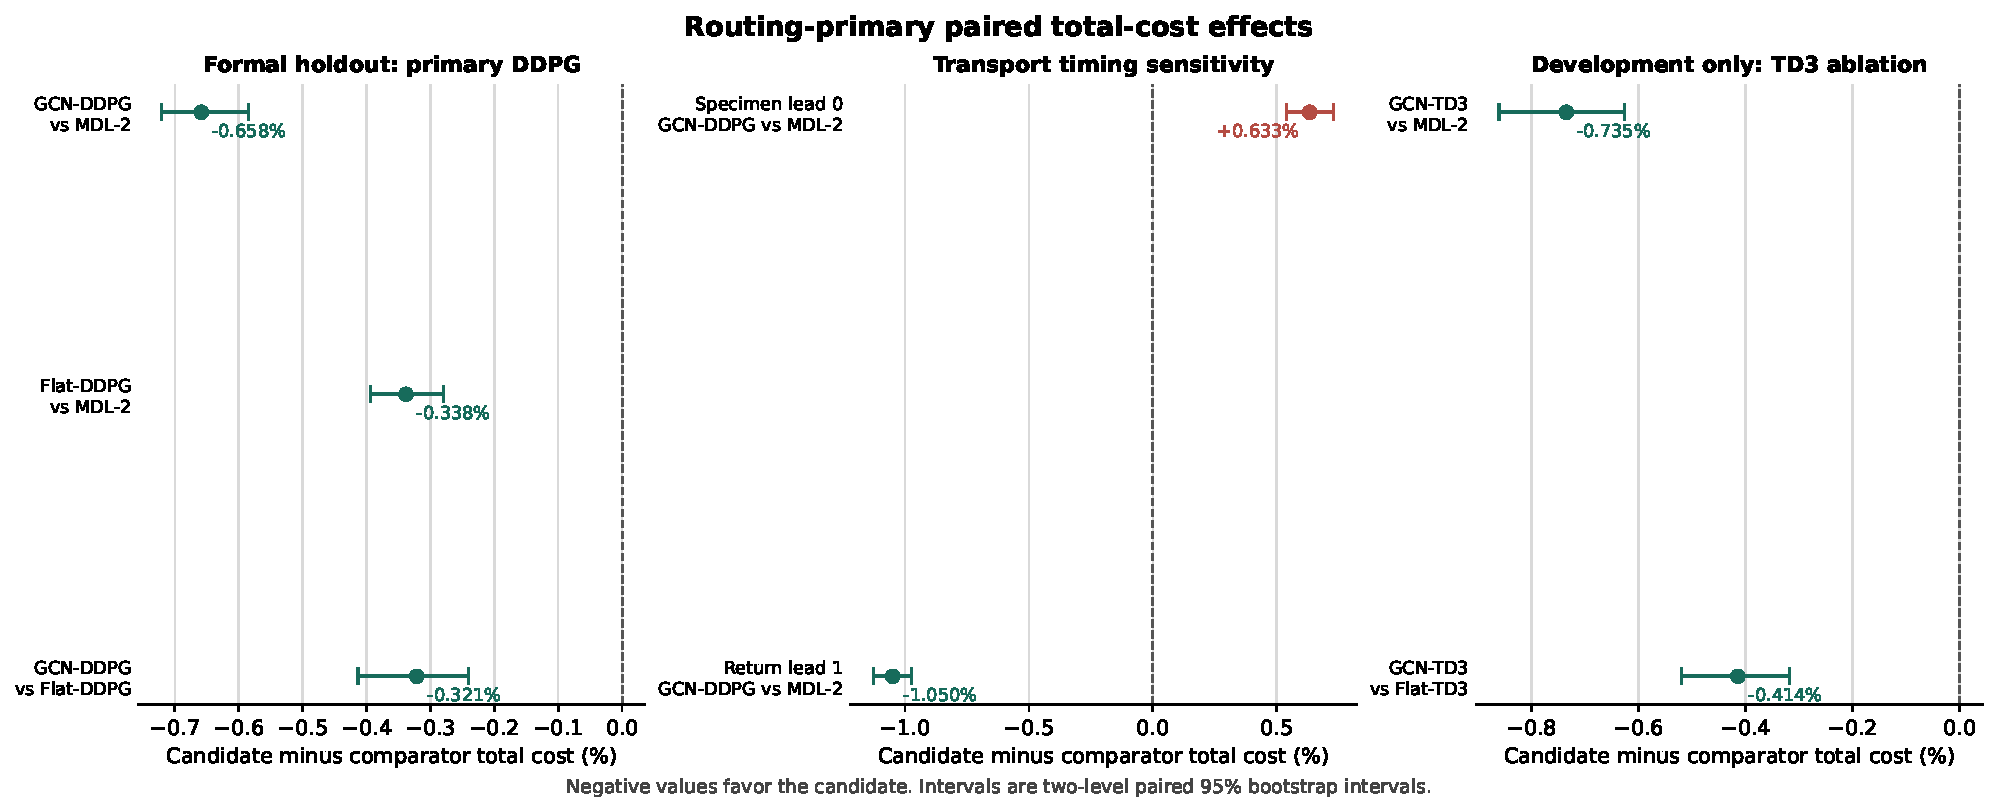
\includegraphics[width=\textwidth]{routing_primary_cost_effects.pdf}
    \caption{Routing-primary paired total-cost effects. Negative values favor
    the candidate, and bars are two-level paired 95\% bootstrap intervals.
    The left panel is formal holdout evidence. The center panel is frozen-policy
    transport-timing sensitivity. The right panel is a development-only TD3
    backbone ablation and is not pooled with the formal result.}
    \label{fig:routing_primary_cost_effects}
\end{figure}

The MDL-2 mean objective is 2,686.444 million units. Its additive components
are base operating cost (45.856\%), patient-loss cost (44.841\%), expiry cost
(8.966\%), and urgency cost (0.337\%). The GCN improvement decomposes into
$-2.100$, $-12.631$, $-2.806$, and $-0.152$ million units for these four
components, respectively. Within base operating cost, specimen-transfer cost
increases by 0.174 million while the remaining operating and shortage
subcomponents decrease by 2.275 million. Specimen transfer is therefore a
mechanistic subcomponent of base cost and is not added to the four-component
total a second time. The dominant benefit is lower modeled patient-loss cost,
not direct transportation savings. Figure~\ref{fig:routing_primary_cost_components}
keeps the additive objective decomposition separate from its base-cost detail.

\begin{figure}[htbp]
    \centering
    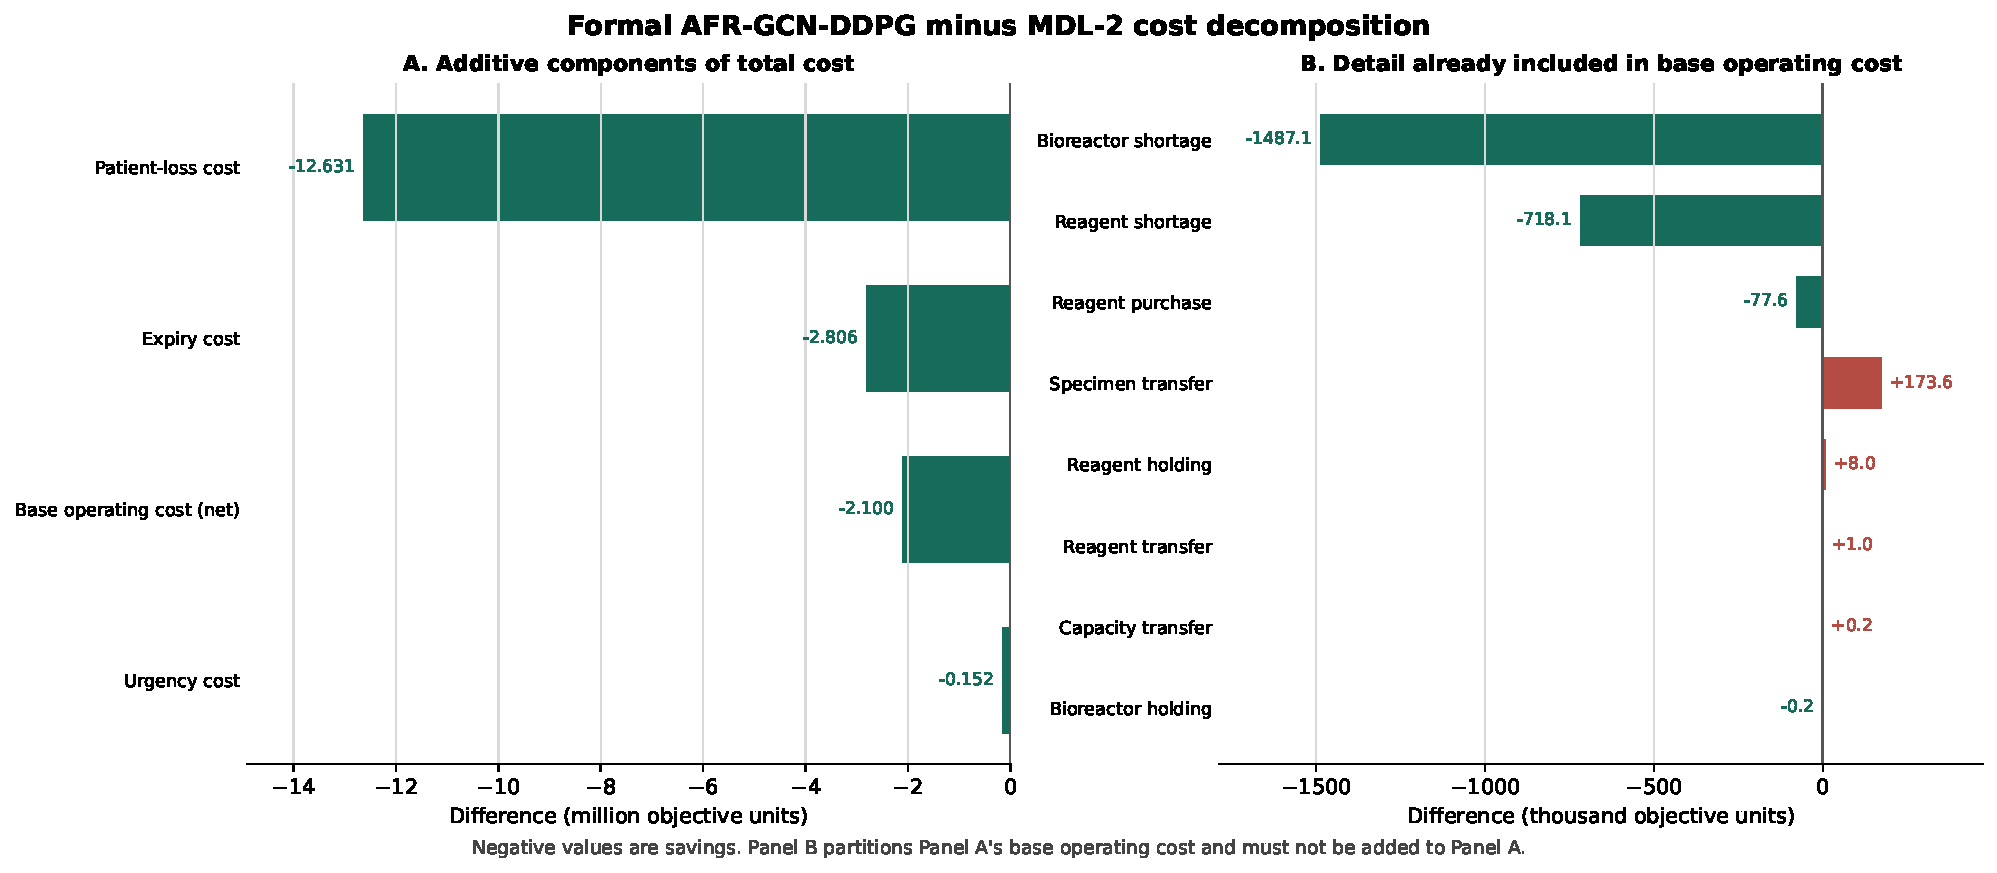
\includegraphics[width=\textwidth]{routing_primary_cost_components.pdf}
    \caption{Formal AFR-GCN--DDPG minus MDL-2 cost decomposition. Negative
    values are savings. Panel A contains the four components that add to total
    cost. Panel B partitions panel A's base operating cost; it is shown for
    mechanism interpretation and must not be added to panel A.}
    \label{fig:routing_primary_cost_components}
\end{figure}

The transport-timing result is asymmetric rather than uniformly robust. When
specimens become available immediately (lead 0 rather than lead 1), GCN cost is
0.633\% higher than MDL-2 and 0.255\% higher than flat. With a one-epoch
finished-product return delay, GCN is 1.050\% lower than MDL-2 and 0.303\%
lower than flat. These are epoch-level availability assumptions, distinct from
continuous geographic travel time, and the reversal precludes a blanket
transport-timing robustness claim.

Finally, the formal final-minus-frozen GCN point estimate is $+0.073$ million
units ($+0.00273\%$), indicating no material online increment. On the separate
paired development checkpoint curve, episode 100 minus episode 75 is $+0.069$
million with interval $[-0.345,+0.502]$ million. Howard's matched three-seed
TD3 development ablation corroborates graph and anchor value: final GCN--TD3 is
0.735\% lower cost than MDL-2 and 0.414\% lower than flat TD3. However, final
GCN--TD3 is 0.00080\% worse than its frozen-pretraining checkpoint, and its
audited paired interval crosses zero. A subsequent structured specimen-option
exploration screen achieved the intended action coverage but produced a GCN
final-minus-frozen effect of $+0.00416\%$ with interval
$[-0.02766,+0.04091]\%$. Thus neither actor--critic backbone establishes an
independent online-learning gain at the tested budget.

\subsubsection{Prospective online-DDPG attribution and action-geometry audits}

The final-versus-frozen comparisons above motivated a prospective DDPG
attribution experiment rather than another unconstrained tuning cycle. Stage F1
created tensor-identical control and candidate forks with the same structured
specimen exploration. The sole candidate difference was an auxiliary
counterfactual-advantage critic loss computed from exact within-state,
four-step behavior-versus-MDL-2 rollouts. All 12 training jobs completed 100
online episodes, and the two prespecified checkpoint curves contained 3,600
learned and 3,600 anchor outcomes in total.

For the primary GCN arm, candidate final minus its frozen pretraining
checkpoint was $-21{,}298$ modeled objective units ($-0.001067\%$), with paired
95\% interval $[-715{,}371,+527{,}375]$. Only one of three seeds was favorable,
so the prospective two-seed and wholly-below-zero gate failed. Candidate final
minus matched control final was $+4{,}081$ units ($+0.000205\%$), with interval
$[-95{,}056,+95{,}036]$ and 131 exact ties among 150 pairs. The auxiliary
target was sampled and partly learned (persisted sign accuracy 0.709--0.786),
but contributed only 0.245--0.343\% of total critic loss and did not produce a
materially different deployed policy.

Read-only transfer audits then examined why additional critic structure did not
reach execution. In the nominal-history G0 diagnostic, the candidate final
critic selected the independently rolled-out best remaining-horizon legal
action in 3/27 states, versus 2/27 for control; only 2/27 raw actor differences
survived correction composition, projection, and integer-lot execution. An
all-legal-action, remaining-horizon ranker in G1 reached 47/156 held-out-seed
top-1 decisions, versus 46/156 for the frozen critic. The original F0/G0/G1
scenario-specific labels were subsequently corrected because those post-hoc
audits had reconstructed nominal history rather than the assigned online
scenario. Their immutable rows remain useful mechanism diagnostics, but no
persistent-hotspot or per-cluster inference is made from them.

Corrected prospective action-geometry screens reconstructed the benchmark-plan
scenarios directly. Table~\ref{tab:action_geometry} reports the
fraction of audited states with an independently validated action saving at
least one million modeled objective units without worsening completion,
patients lost, or manufacturing ineligibility. Specimen routing retained local
headroom, whereas neither continuous resource group produced a prospectively
selected material improvement.

\begin{table}[htbp]
\centering
\caption{Corrected frozen action-geometry screen. H0 is the persistent-shift
screen and H1 is the nonstationary screen. ``Opp.'' is the fraction of 27
audited states with a material clinically noninferior action; ``selected''
applies the same test to the action chosen on an independent discovery stream.}
\label{tab:action_geometry}
\begin{tabular}{lrrrr}
\hline
Action group & H0 opp. & H0 selected & H1 opp. & H1 selected \\
\hline
Specimen transfer & 55.6\% & 40.7\% & 55.6\% & 37.0\% \\
Reagent transfer & 3.7\% & 0.0\% & 3.7\% & 0.0\% \\
Reagent plus capacity & 3.7\% & 0.0\% & 0.0\% & 0.0\% \\
\hline
\end{tabular}
\end{table}

Together, these audits narrow rather than erase the reinforcement-learning
contribution. The learned graph residual policy is supported by the formal
policy comparisons and the TD3 backbone ablation. What is not supported is a
separate claim that the tested online Bellman and policy-gradient updates
created the endpoint gain. In the current simulator, useful local control
authority is concentrated in projected discrete specimen choices, while the
channels that preserve continuous action geometry expose little clinically
noninferior material headroom.

\section{Discussion and Conclusions}
\label{sec:conclusion}
This study develops a patient-condition and geography-aware simulation of a
20-clinic PRM network, including identity-preserving pre-manufacturing specimen
routing, and a residual GCN--DDPG controller that learns around a
strong MDL-2 anchor. Advantage-filtered distillation identifies sparse
state-dependent corrections, while checkpoint selection, residual-scale
calibration, and fallback prevent an unsupported correction from being
deployed. This structure preserves the interpretability of the anchor while
allowing the graph actor to respond to patient pressure, transfer pipelines,
regional disruptions, and demand-prior drift.

The routing-primary formal result now supplies the main controller evidence.
With routing held admissible for all policies, AFR-GCN--DDPG improves on both
routing MDL-2 and a parameter-matched flat controller, and all reported
patient-facing metrics move in the favorable direction. The graph-versus-flat
interval is wholly below zero, so this matched experiment supports a
graph-representation advantage rather than only generic residual learning.
Routing itself is not the treatment in this comparison; estimating the value
of making routing admissible would require a separately locked routing-versus-
no-routing design.

The component analysis also changes the interpretation of the result. Lower
patient-loss cost accounts for most of the total reduction, followed by expiry
and net operating cost. Specimen-transfer cost rises, as expected when a graph
controller makes greater use of geographic reallocation, but this increase is
more than offset by reductions elsewhere. Reporting the component changes
alongside the full-objective percentage preserves the preregistered denominator
and shows that the gain is patient- and shortage-facing rather than an artifact
of inexpensive transport.

The method attribution is narrower than the policy comparison. Frozen
advantage-filtered pretraining already captures nearly all observed DDPG and
TD3 value. The prospective F1 paired-critic experiment also failed its
final-versus-frozen and candidate-versus-control gates. Mechanism audits found
weak long-horizon legal-action ranking, severe attenuation through projection
and integer-lot execution, and little clinically noninferior headroom in the
simulator's genuinely continuous resource channels. We therefore distinguish
three supported layers: the constrained graph-MDP formulation, the
advantage-filtered graph residual policy class, and its calibrated execution
pipeline. The formal evidence supports the complete learned controller and a
graph-versus-flat advantage; it does not establish an independent contribution
from the tested online actor--critic updates. DDPG remains the canonical
backbone because it is the prespecified five-seed formal method. The matched
TD3 result is a useful development ablation, not evidence that DDPG generally
dominates TD3 or that TD3 has formal-holdout status.

This attribution result also yields a reusable experimental design rule. Before
committing another actor--critic campaign to a candidate decision channel, the
channel should first demonstrate four properties on independent simulation
streams: clinically noninferior headroom beyond the incumbent anchor, value
from conditioning on decision-time state rather than using a tuned constant,
stable counterfactual action labels, and behavioral sensitivity after decoding
and feasibility projection. Failure of any one property makes an endpoint
online-RL gain difficult to identify even when optimization diagnostics are
finite and the policy network changes. Treating these checks as prospective
admissibility gates is a methodological lesson from the negative attribution
evidence, not a claim that another policy has already passed them.

Several limitations remain. The routing-primary DDPG comparison has five
training seeds, but the matched TD3 and mechanism-diagnostic screens have only
three and use development streams. The formal comparison isolates graph versus
flat representation and policy versus MDL-2, but it does not isolate routing
availability or the incremental contribution of online updates. F1 and the
corrected H0/H1 action-geometry screens use three training seeds and bounded
state samples; they reject their prespecified advancement gates but do not
prove that every possible online algorithm or continuous action is ineffective.
The original F0/G0/G1 post-hoc rows reconstruct nominal history, so their former
scenario-specific labels are superseded and only their mechanism-level
diagnostics are retained. Transport
timing is not uniformly robust, and continuous travel-time viability is not
coupled to the epoch-level availability sensitivity. Pure-policy, SAC, and PPO
controllers have not been evaluated under the same locked routing-primary
budget and should not be ranked from these data. The clinical calibration
target is literature aligned but is not fitted to patient-level data from a
single indication, so sensitivity bands remain necessary. Patient-loss,
expiry, urgency, and shortage coefficients are modeled decision weights rather
than a complete accounting valuation; external economic and clinical
calibration is required before interpreting objective differences as realized
monetary savings or deploying the controller operationally.
The routing-capable environment has passed implementation-level identity,
conservation, lifecycle, and CRN tests, and the five-seed routing-primary
GCN/flat confirmation is complete. Its formal claim is about controllers under
a common routing-capable environment, not about the causal value of routing.
Transport-timing sensitivity is asymmetric, with the primary advantage
reversing under immediate specimen availability, so general timing robustness
is not claimed. Development-only TD3 and DDPG mechanism screens remain labeled
and archived separately from formal holdout evidence.

\textbf{Future Work}
This study motivates several extensions. Patient condition can be represented
with longitudinal clinical covariates rather than the current eligibility and
survival-risk summary. Raw-material quality, product quality, process failures,
machine breakdowns, and operator availability can be added to the simulator.
The completed routing-primary protocol and its evidence map should now remain
frozen. Future empirical work should use new research questions and independent
streams rather than repeatedly tuning online attribution on the existing
development evidence. Valuable extensions include unseen clinic networks,
continuous transport-viability coupling, transfer disruptions, externally
calibrated economic weights, and a separately prespecified routing-versus-no-
routing study. If online deterministic policy gradients are to be made central,
a new model should expose stable continuous operational authority with genuine
intertemporal consequences. A promising example is advance staffing or
overtime-capacity commitment with ramping delays, convex fatigue or activation
costs, and persistent carryover, rather than a scalar same-epoch adjustment.
Any production-rate or procurement extension should first verify that its
effect remains continuous after execution and is not removed by integer-lot
rounding or absorbed by a tuned look-ahead anchor. Such a study requires a
separate preregistration, new comparators, independent streams, and the four
admissibility gates above; it is not an extension of the frozen formal result.
Longer-term models should integrate production scheduling,
product preparation and distribution, and treatment operations.

\section*{Data Availability}
All study data are generated by the simulation model. The accompanying
repository contains the source code, locked experiment configurations, curated
summary outputs, training diagnostics, artifact hashes, and a claim-to-evidence
map. Large checkpoint tensors and row-level Monte Carlo files are omitted from
version control but are SHA256-inventoried and available from the corresponding
author upon reasonable request.

\section*{Declaration of Competing Interest}
The author declares that there is no known competing financial interest or personal relationship that could have appeared to influence the work reported in this paper.

\printbibliography

\end{document}
